%% WiNN supplementary material for Bioinformatics
%% WiNN 0.1.6 benchmark analyses (frozen 11 November 2026)

\documentclass[namedate,webpdf,modern,large,nocrop]{oup-authoring-template}
\graphicspath{{figures/supplementary_panels/}}
\newcommand{\societylogo}{}
\usepackage{array}
\usepackage{booktabs}
\usepackage{float}
\usepackage{longtable}
\usepackage{microtype}
\usepackage{multirow}
\usepackage{pdflscape}
\newcommand{\supppanel}[2]{\begin{minipage}[t]{#1}\centering\includegraphics[width=\linewidth]{#2}\end{minipage}}

\begin{document}
\journaltitle{Bioinformatics}
\copyrightyear{2026}
\pubyear{2026}
\access{Supplementary material}
\appnotes{Original Paper}
\firstpage{1}
\title[WiNN supplementary material]{Supplementary material for: WiNN enables selective correction of run-order drift and batch effects in metabolomics data}
\author[1,2,6]{Tanmay Tanna}
\author[2]{Yirui Zhang}
\author[2]{Anja Sjöström}
\author[4]{Franco Giulianini}
\author[2,6]{Malte Londschien}
\author[2]{Antoine Jeanrenaud}
\author[2,5,8]{André Kahles}
\author[7]{Mitchell P. Levesque}
\author[2,5,6,8,$\ast$]{Gunnar Rätsch}
\author[2,3,4,$\ast$]{Olga Demler}
\address[1]{\orgdiv{Department of Biosystems Science and Engineering}, \orgname{ETH Zürich}, \orgaddress{\country{Switzerland}}}
\address[2]{\orgdiv{Department of Computer Science}, \orgname{ETH Zürich}, \orgaddress{\country{Switzerland}}}
\address[3]{\orgdiv{Harvard T.H. Chan School of Public Health}, \orgaddress{\state{MA}, \country{USA}}}
\address[4]{\orgdiv{Brigham and Women's Hospital, Harvard Medical School}, \orgaddress{\state{MA}, \country{USA}}}
\address[5]{\orgdiv{Medical Informatics}, \orgname{University Hospital Zürich}, \orgaddress{Zürich, \country{Switzerland}}}
\address[6]{\orgname{AI Center, ETH Zürich}, \orgaddress{Zürich, \country{Switzerland}}}
\address[7]{\orgdiv{Department of Dermatology}, \orgname{University Hospital Zürich and Medical Faculty, University of Zürich}, \orgaddress{\country{Switzerland}}}
\address[8]{\orgname{Swiss Institute for Bioinformatics}, \orgaddress{\state{Lausanne}, \country{Switzerland}}}
\corresp[$\ast$]{Corresponding authors. \href{mailto:raetsch@inf.ethz.ch}{raetsch@inf.ethz.ch}; \href{mailto:odemler@bwh.harvard.edu}{odemler@bwh.harvard.edu}}
\abstract{Detailed algorithms, benchmark designs, complete benchmark results, uncertainty analyses, ablations and numerical validation supporting the main manuscript.}
\keywords{metabolomics; mass spectrometry; run-order drift; batch effects; normalization; supplementary methods}
\onecolumn
\maketitle

\setcounter{section}{0}
\setcounter{figure}{0}
\setcounter{table}{0}
\renewcommand{\thesection}{S\arabic{section}}
\renewcommand{\thesubsection}{\thesection.\arabic{subsection}}
\renewcommand{\thefigure}{S\arabic{figure}}
\renewcommand{\thetable}{S\arabic{table}}

\section*{Supplementary Methods}

\section{WiNN algorithm}
\label{sec:supp_algorithm}

\subsection{Input, robust preparation and analysis scale}

Let \(X=(x_{ij})\in\mathbb{R}_{\geq0}^{p\times n}\) contain \(p\) features and \(n\) sequential injections. Injection \(j\) has run order \(t_j\) and a supplied or inferred acquisition segment \(b(j)\). Quality-control (QC) reference samples are repeated injections of reference material used for tuning or evaluating analytical precision. For feature \(i\), WiNN calculates
\[
m_i=\operatorname{median}_{j}(x_{ij}),\qquad d_i=\operatorname{MAD}_{j}(x_{ij}).
\]
Here \(d_i\) is R's scaled MAD, using the default consistency constant 1.4826. The primary \texttt{winn()} entry point requires finite, non-negative intensities. The standalone \texttt{adjust\_outliers\_mad()} helper permits nonfinite values; these are excluded from threshold estimation and returned unchanged, while later nonfinite test or fit results are handled conservatively as described below. For finite observations, values at or beyond \(m_i\pm4d_i\) are flagged. The median, MAD, both thresholds and both masks are calculated once from the original finite observations, after which upper and lower flags are mapped independently into their respective 3--4 MAD bands in one non-iterative pass. Values within the thresholds are left unchanged; values outside them are not removed, but are monotonically shrunk toward the interior of the distribution by linear interpolation. Features with zero or undefined MAD remain unchanged. Tests and correction models use \(z_{ij}=\log(1+\widetilde x_{ij})\), where \(\widetilde x_{ij}\) is the prepared intensity. Shrinkage is used in place of outlier exclusion to limit undue leverage on downstream inference while preserving informative extreme observations; it also limits rare biological responses that fall beyond the thresholds.

\subsection{Feature-segment run-order gate}

For metabolite \(i\) and segment \(s\), containing \(n_s\) injections, WiNN tests the null hypothesis that the ordered values \(\{z_{ij}: j\in s\}\) are consistent with white noise along run order. By default, the test statistic is the Ljung-Box statistic \citep{LjungBox1978}
\[
Q_i^{(s)}(h_s)=n_s(n_s+2)\sum_{\ell=1}^{h_s}\frac{\widehat\rho_{i\ell}^{(s)2}}{n_s-\ell}.
\]
Here \(\widehat\rho_{i\ell}^{(s)}\) is lag-\(\ell\) autocorrelation. Let \(d_{\mathrm{fit}}\) denote the Ljung-Box fitted-model degrees of freedom and define \(h_{\min}=d_{\mathrm{fit}}+3\). If \(n_s-1<h_{\min}\), the profile is not tested and remains unchanged. Otherwise, when no lag is supplied,
\[
h_s=\min\!\left\{n_s-1,\max\!\left[h_{\min},\min\!\left(10,\left\lfloor n_s/5\right\rfloor\right)\right]\right\}.
\]
A user-supplied lag is likewise raised to at least \(h_{\min}\) and capped at \(n_s-1\). The primary configuration uses \texttt{fitdf=0}, because no ARMA model is fitted before testing, so \(h_{\min}=3\) and the approximate reference chi-square distribution has \(h_s\) degrees of freedom. The gate is a heuristic screen for serial dependence across all injections; its nominal BH threshold does not establish finite-sample FDR control. Its interpretation depends on the acquisition design: scheduled reference types and repeated identities can produce serial dependence independently of instrumental drift. Finite-sample calibration is evaluated in Section~\ref{sec:supp_targeted_revision}. Profiles producing a nonfinite test result are retained without detrending. Durbin-Watson testing is available as an alternative \citep{DurbinWatson1951}. Benjamini-Hochberg adjustment is performed across features within each segment, giving one testing family per segment \citep{BenjaminiHochberg1995}.

Only selected feature-segment profiles are detrended. The primary configuration uses the conservative smoother hierarchy. For \(n_s<5\), WiNN fits a linear model. For \(n_s\geq5\), it sets \(k_s=\max\{4,\min(10,\lfloor n_s/5\rfloor)\}\) and attempts, in order, a P-spline generalized additive model (GAM) with \(k=k_s\), REML estimation and \(\gamma=1.4\); a thin-plate GAM with \(k=k_s\), REML estimation and \(\gamma=1.2\); a fixed cubic-regression spline with \(k=\min(6,k_s)\) and \texttt{fx=TRUE}; LOESS with span 0.3 and degree 1; and linear regression \citep{Cleveland1979LOESS,Wood2017GAM}. The separate standard option fits \(z\sim s(t,\mathrm{bs}=\texttt{"cr"})\) and falls back to a linear model. If spline fitting fails, WiNN falls back successively to simpler smoothers, ultimately to a linear trend, and a profile remains unchanged if no fit returns finite fitted values. For fitted curve \(\widehat f_i^{(s)}\),
\[
z_{ij}^{\mathrm{drift}}=z_{ij}-\left\{\widehat f_i^{(s)}(t_j)-\overline{\widehat f_i^{(s)}}\right\},\qquad
\overline{\widehat f_i^{(s)}}=n_s^{-1}\sum_{j\in s}\widehat f_i^{(s)}(t_j).
\]
Centering ensures that detrending preserves the segment mean on the transformed scale. The forced-drift ablation fits the same correction to every testable profile and bypasses only the gate.

\subsection{Residual batch gate}

After detrending, WiNN fits \(z_{ij}^{\mathrm{drift}}=\mu_i+\beta_{i,b(j)}+\varepsilon_{ij}\) feature by feature. ANOVA \(P\)-values are BH-adjusted across features. A selected feature receives
\[
z_{ij}^{\mathrm{batch}}=z_{ij}^{\mathrm{drift}}-\overline z_{i,b(j)}^{\mathrm{drift}}+\overline z_i^{\mathrm{drift}}.
\]
This removes batch-specific location shifts while preserving the global metabolite mean. An eligible feature is a retained row whose \(\log(1+x)\) values are finite across all injections, and the stage is skipped when fewer than two batch levels are present. ANOVA is attempted for every eligible feature, but selective correction requires a finite BH-adjusted \(P\)-value below the nominal false-discovery rate (FDR) threshold; a non-estimable result is not selected. The forced-batch ablation applies the same location-shift correction to every eligible feature. An empirical-Bayes ComBat branch is available, but the primary configuration uses the ANOVA branch \citep{Johnson2007ComBat}.

\subsection{Conservative probabilistic quotient normalization}

All PQN calculations are performed after inverse transformation to the non-negative intensity scale. For reference set \(C\), WiNN calculates \(r_i=\operatorname{median}_{j\in C}x_{ij}^{\mathrm{batch}}\). The primary configuration sets \texttt{control\_samples=NULL}, so \(C\) contains all injections; QC-tuned configurations use labelled training controls. Only features with \(r_i>0\) contribute to quotient estimation:
\[
q_{ij}=x_{ij}^{\mathrm{batch}}/r_i,\qquad d_j=\operatorname{median}_{i:r_i>0}(q_{ij}).
\]
Features with zero reference medians are omitted from dilution-factor estimation but remain in the returned matrix. Let \(\bar d\) and \(s_d\) be the arithmetic mean and standard deviation of the positive dilution factors. Conservative PQN leaves sample \(j\) unchanged when \(d_j\in[\bar d-s_d,\bar d+s_d]\); otherwise all intensities in that sample are multiplied by \(b_j/d_j\), where \(b_j\) is the nearest boundary of that interval. Thus, injections within the central range are left unchanged, whereas only extreme dilution factors are shrunk back toward the bulk of the cohort. Full PQN instead divides every sample by \(d_j\) \citep{Dieterle2006PQN}. PQN estimates dilution from median feature quotients and therefore assumes that most features are unaffected by a coordinated biological response. Within-segment standardization is optional and was disabled in the benchmarks. WiNN returns the full feature panel together with gate decisions and diagnostics.

\subsection{Benchmarked configurations and automatic segmentation}

Throughout the manuscript, tables and figures, \emph{WiNN} denotes the prespecified primary configuration with supplied batch labels and no QC-guided tuning. It uses \texttt{parameters="fixed"}, supplied segments, \texttt{control\_samples=NULL}, MAD preparation, adaptive-lag Ljung-Box testing with \texttt{fitdf=0} at a BH-adjusted threshold of 0.05, conservative smoothing, residual-batch ANOVA at a BH-adjusted threshold of 0.05 and conservative PQN. It receives no QC identities and performs no parameter search.

When configurations are compared directly, \emph{WiNN (QC-tuned)} denotes the option that retains supplied batch labels and uses labelled training controls to select from prespecified nominal drift thresholds \(\{0.10,0.05,0.01\}\), nominal batch thresholds \(\{0.10,0.05,0.01\}\), supported serial-dependence tests, standard or conservative smoothers and conservative or full PQN (Table~\ref{tab:supp_selected_parameters} reports the package values \texttt{shrink} and \texttt{normalize} as conservative and full PQN). Candidate pipelines are scored using control-only agreement and variability criteria, so controls are used for model selection and evaluation, not for direct drift fitting: run-order smooths are fitted to the complete within-segment profile, in which control injections appear as ordinary observations.

\emph{WiNN (inferred segments)} combines the same QC-guided tuning with inferred acquisition segments. It first infers contiguous acquisition segments by functional-pruning changepoint detection applied to \(a_j=\operatorname{median}_{i}(\widetilde x_{ij})\). It minimizes
\[
\sum_{k=0}^{K}\mathcal C\!\left(a_{(\tau_k+1):\tau_{k+1}}\right)+\beta K
\]
over boundaries \(0=\tau_0<\tau_1<\cdots<\tau_{K+1}=n\). Long segments use sparse natural-spline means; short segments use constant means. The default modified-BIC penalty is \(3\log n\) \citep{Killick2012PELT,Maidstone2017FPOP}. Inferred versus supplied segment counts were 2 versus 5 in simulation, 3 versus 8 in MTBLS79, 2 versus 8 in the clinical dataset, 6 versus 10 in BatchCorr, 3 versus 2 in Sacurine and 1 versus 3 in WaveICA. When segments are inferred from the same data, the subsequent \(P\)-values are interpreted conditionally on that estimated segmentation and are not intended as a full post-selection error-control guarantee. Supplied segments remain the recommended input. The API also permits fixed parameters with omitted batch labels, which invokes automatic segmentation before the fixed correction sequence; this combination was not reported as a separate benchmark output.

\section{Benchmark designs}
\label{sec:supp_designs}

\subsection{Canonical truth-known simulation}

Each seed contains 1,000 features and 500 injections in five plates of 100. Ninety study samples and ten pooled QCs occur per plate; QCs are interleaved every ten acquisitions. Ten QCs are selected before fitting as label-blinded references, leaving 40 labelled training QCs. Clean study log intensities are independent draws from \(N(0,0.35^2)\). QCs share one clean reference profile.

Plate-effect susceptibility is drawn independently with probability 0.70. Conditional on assignment, feature-plate offsets are Gaussian draws with standard deviation 0.60, except for a further Bernoulli 0.10 subset drawn with standard deviation 1.35; offsets are then centered across plates. Run-order susceptibility is drawn with probability 0.60. For each susceptible feature, plate-specific activity is sampled with probability 0.55, with at least one active plate. Active profiles use linear, nonlinear, autoregressive or mixed trajectories. Each trajectory is centered and scaled to a maximum log-amplitude drawn uniformly from 0.20 to 0.85. If \(G\), \(B\) and \(D\) denote clean, plate-offset and drift matrices on the log scale, observed intensities are \(X=\exp(G+B+D)\). Ten independent component-seed sets were completed for every method.

\subsection{Partial-confounding simulation}

The confounding experiment reuses the canonical technical artifacts and adds a balanced binary phenotype to the 450 study injections. One hundred features are selected once per master seed; 50 receive a case-control log effect of (+0.35), 50 receive (-0.35), and all remaining features receive zero. Centered phenotype coding gives 225 cases and 225 controls without changing the study grand mean. Pooled QCs receive no biological effect. Phenotype labels and response truth are excluded from correction metadata.

The zero-strength allocation places 45 cases in each plate using fixed random priorities. Batch alignment moves plate case counts toward the maximum feasible pattern \((90,90,45,0,0)\). Run-order alignment swaps late cases with the earliest controls within each plate while retaining 45 cases per plate. Joint alignment applies both rules. Strengths are 0.25, 0.50, 0.75, 0.90 and 1.00; zero is represented once, giving 16 scenarios per seed and 160 scenario-seed tasks. Strength 1 is the most aligned arrangement allowed by this balanced five-plate design, not complete separation of phenotype from all technical variables.

\subsection{Empirical datasets and independent units}

MTBLS79 is a repeated-sample direct-infusion mass-spectrometry benchmark with 2,488 features, 172 injections and eight batches \citep{Kirwan2014DIMSBenchmark}. It contains 134 study injections from 20 extracts, ten cow and ten sheep, plus 38 pooled references. Twelve references are label-blinded.

BatchCorr Set 1 contains 710 \emph{Arabidopsis} study injections and 51 pooled references across ten batches \citep{Wehrens2016BatchCorr}. The study injections represent 357 accessions, including 346 observed in multiple batches. Ten references are label-blinded. Variables observed in fewer than 80\% of samples are removed. This leaves 199 features and 3.11\% missing values, imputed with \texttt{missForest} using seed 42 \citep{Stekhoven2012missForest}.

The internal clinical serum metabolomics cohort was acquired by FIA-MS ToF using a 96-well plate design optimized to separate technical from biological variation \citep{Fuhrer2011FIATOF}. Study samples were distributed across plates under explicit randomization constraints, while preserving within-patient longitudinal structure by placing time-course samples adjacently but in an order unrelated to collection time. To reduce confounding between acquisition order and sample metadata, plate layouts were iteratively re-randomized and assessed using $\chi^2$ tests across plates and plate blocks and Runs tests on within-plate sample sequences. Pooled QC material, generated from a random subset of study samples, was inserted every eighth well, and each biological sample was prepared on two plates and injected twice per plate, yielding four technical measurements per sample. Blank wells and NIST1950 reference injections were also included on each plate to assess analytical stability, repeatability and residual plate effects. The resulting dataset contains 1,594 features and 1,320 injections across eight plates. Injections form 660 adjacent, within-plate technical pairs: 536 clinical pairs, 86 training-control pairs and 38 label-blinded NIST1950 pairs. Each method is fitted to pair-level \(\log(1+x)\) means. The learned log correction is applied identically to both original injections in a pair. The 536 study pair means represent 267 biological identities observed across plates. Plate \(R^2\) and biological identity metrics use only these study pairs; held-out CV uses the 38 masked NIST pairs. No phenotype or disease endpoint is used.

Sacurine contains 184 human urine study injections, 26 pooled QCs, 113 metabolites and two batches \citep{Thevenot2015Sacurine,Thevenot2018W4M00001}. Files were pinned from the \texttt{phenomis} mirror at commit \texttt{1e83ce6}; eight QCs are label-blinded. Age, BMI, gender, sampling factor and osmolality are withheld from correction. Correction and technical endpoints use the unscaled deposited matrix. For biological endpoints only, each corrected study profile is divided by its sample osmolality before $\log(1+x)$ transformation, which keeps osmolality outside the correction procedure.

WaveICA contains an XCMS-derived human plasma peak table with 6,461 peaks, 568 study injections, 74 pooled QCs and three batches \citep{Smith2006XCMS,Deng2021WaveICA}. Fifteen QCs are label-blinded. The study labels are retained as \texttt{group\_0} and \texttt{group\_1}, containing 71 and 497 samples. The labels are not mapped to a diagnosis.

\begin{table*}[tbp]
\centering
\small
\caption{Benchmark structure and independent evaluation units. Hidden references remain in the intensity matrix with their identities masked, giving label-blinded, transductive evaluation.}
\label{tab:supp_design}
\begin{tabular}{lrrrrrrp{4.3cm}}
\toprule
Dataset & Features & Injections & Study units & References & Batches & Hidden refs. & Independent biological unit or anchor \\
\midrule
Simulation & 1,000 & 500 & 450 & 50 & 5 & 10 & Study injection; clean matrix; ten seeds \\
MTBLS79 & 2,488 & 172 & 134 & 38 & 8 & 12 & Twenty cow or sheep extracts with repeats \\
BatchCorr Set 1 & 199 & 761 & 710 & 51 & 10 & 10 & 357 accessions, 346 repeated across batches \\
Clinical FIA-MS & 1,594 & 1,320 & 536 log-pair means & 124 control pairs & 8 & 38 & 267 biological identities across plates \\
Sacurine & 113 & 210 & 184 & 26 & 2 & 8 & Study sample; age, BMI and gender \\
WaveICA & 6,461 & 642 & 568 & 74 & 3 & 15 & Study sample; deposited group 0 or 1 \\
\bottomrule
\end{tabular}
\end{table*}

\section{Correction methods and selection protocol}
\label{sec:supp_methods}

Reference panels were selected once before fitting. Their metadata QC identities were replaced by ordinary study labels; their intensity columns remained in each matrix as unlabeled observations. This is a transductive design: a masked column can affect a correction fitted to all injections even when its QC identity is withheld. Biological labels, replicate identities, batch-separation results and final evaluation ranks are absent from every selection record.

Raw data, ComBat, QC-RLSC, QC-RFSC, TIGER, SERRF and three WiNN modes are evaluated. Candidate sets and seeds are frozen before evaluation. Training-QC selection uses only labelled training-QC intensities, identities, run order and supplied batches. Endpoint comparisons use the same ordered sample and feature identifiers across methods. All outputs retain the declared feature and sample panel. Raw-value fallbacks and other numerical safeguards are summarized in Section~\ref{sec:supp_audit_results}.

ComBat uses \texttt{sva} 3.56.0 \citep{Johnson2007ComBat}. The selection manifest records a two-candidate training-QC search over \texttt{par.prior} for MTBLS79, BatchCorr and the clinical cohort: the selected setting is parametric (\texttt{TRUE}) in MTBLS79 and BatchCorr and nonparametric (\texttt{FALSE}) in the clinical cohort. Simulation, Sacurine and WaveICA use the prespecified parametric setting without search. The correction model itself uses supplied batches; the training QCs in those three datasets inform configuration selection. QC-RLSC uses an identifier-safe per-batch LOESS fit trained only on labelled controls, followed by interpolation to study injections \citep{Dunn2011,Cleveland1979LOESS}; this direct implementation was used because the \texttt{qcrlscR::qc.rlsc.wrap()} wrapper did not reliably propagate the intended span and order settings. QC-RFSC uses \texttt{statTarget} 1.38.0 \citep{Luan2018StatTarget}. TIGER uses \texttt{TIGERr} 1.0.2 with its native \(4\times4\) ensemble and 500 trees \citep{Han2022TIGER}. SERRF uses \texttt{malbacR} 0.1.0 \citep{Fan2019SERRF,Leach2023malbacR}. Package defaults or training-QC-selected candidates are recorded for every dataset-method pair in Table~\ref{tab:supp_selected_parameters} and the accompanying exact manifest. The external training-QC candidate score is mean pairwise QC-profile Pearson correlation minus one half of mean feature QC CV expressed as a fraction; higher is preferred. WiNN automatic modes use the package-native QC score and grids specified in Section~S1; their selected settings are included in Table~\ref{tab:supp_selected_parameters}.

\paragraph{QC-RFSC implementation.} The adapter assigns neutral identifiers to every injection, then marks training QCs for \texttt{statTarget}. The detected training indices are checked against the prespecified reference set before each fit. Feature-wise relative outputs are multiplied by the corresponding training-QC median to restore abundance units. Missing or nonfinite feature outputs revert to raw values, with fallback counts recorded. This preserves the input abundance scale for log1p RMSE and multifeature profile comparisons. QC-RFSC simulation results and empirical point estimates use this implementation. Reference-partition, biological-association and empirical bootstrap comparisons include the other eight outputs.

\begin{table*}[tbp]
\centering
\small
\caption{Compared outputs and information available during fitting or selection. All configurations were frozen before final endpoint evaluation.}
\label{tab:supp_methods}
\begin{tabular}{p{2.0cm}p{2.9cm}p{1.0cm}p{1.1cm}p{1.7cm}p{4.8cm}}
\toprule
Output & Implementation & Supplied batches & Training QCs & Search & Selection rule \\
\midrule
Raw & Identity & no & no & no & No correction \\
ComBat & \texttt{sva} 3.56.0 & yes & dataset-specific & 1 or 2 candidates & Prespecified setting or training-QC score; see Table~\ref{tab:supp_selected_parameters} \\
QC-RLSC & Direct LOESS; \texttt{qcrlscR} wrapper not used & yes & yes & dataset-specific & Fixed safeguard or training-QC score \\
QC-RFSC & \texttt{statTarget} 1.38.0 & yes & yes & dataset-specific & Prespecified default or training-QC score \\
TIGER & \texttt{TIGERr} 1.0.2 & yes & yes & native ensemble & Native setting with reliable run order \\
SERRF & \texttt{malbacR} 0.1.0 & yes & yes & dataset-specific & Native setting or training-QC score \\
WiNN (QC-tuned) & \texttt{winn} 0.1.6 & yes & yes & 36 or 72 candidates & Package score using training QCs only \\
WiNN (inferred segments) & \texttt{winn} 0.1.6 & no & yes & 36 or 72 candidates & Segment inference, then training-QC score \\
WiNN & \texttt{winn} 0.1.6 & yes & no & no & One prespecified configuration \\
\bottomrule
\end{tabular}
\end{table*}

\begingroup
\begin{landscape}
\scriptsize
\begin{longtable}{p{2.6cm}p{3.4cm}p{9.6cm}rp{3.6cm}}
\caption{Selected correction settings for every dataset and method. Comparator candidates were prespecified or scored on labelled training QCs only. WiNN (QC-tuned) and WiNN (inferred segments) selected settings from the package grid (36 or 72 candidates; Section~S1) using training QCs only; segment counts are shown in parentheses. WiNN uses one prespecified configuration in every dataset and receives no QC identities. Raw is the identity operation, and TIGER uses its native $4\times4$ ensemble with injection order and 500 trees in every dataset.}\label{tab:supp_selected_parameters}\\
\toprule
Dataset & Method & Selected settings & Candidates & Selection \\
\midrule
\endfirsthead
\multicolumn{5}{l}{\textit{Table \thetable{} continued}}\\
\toprule
Dataset & Method & Selected settings & Candidates & Selection \\
\midrule
\endhead
\midrule
\multicolumn{5}{r}{\textit{Continued on next page}}\\
\endfoot
\bottomrule
\endlastfoot
Simulation & ComBat & par\_prior=TRUE & 1 & Prespecified or native \\
Simulation & QC-RLSC & span=0.75; degree=1 & 1 & Prespecified or native \\
Simulation & QC-RFSC & ntree=500; coCV=30; Frule=0.8 & 1 & Prespecified or native \\
Simulation & SERRF & jitter\_eps=0; documented fallback only after numerical failure & 1 & Prespecified or native \\
Simulation & WiNN (QC-tuned) & batches supplied (5); Ljung-Box; standard smoother; drift FDR 0.10; batch FDR 0.01; PQN conservative & grid & Package training-QC score \\
Simulation & WiNN (inferred segments) & batches inferred (2); Ljung-Box; standard smoother; drift FDR 0.05; batch FDR 0.10; PQN conservative & grid & Package training-QC score \\
Simulation & WiNN & batches supplied (5); Ljung-Box; conservative smoother; drift FDR 0.05; batch FDR 0.05; PQN conservative & 1 & Prespecified \\
\midrule
MTBLS79 & ComBat & par\_prior=TRUE & 2 & Training-QC score \\
MTBLS79 & QC-RLSC & span=0.7; degree=1 & 4 & Training-QC score \\
MTBLS79 & QC-RFSC & ntree=500; coCV=30; Frule=0.8 & 4 & Training-QC score \\
MTBLS79 & SERRF & jitter\_eps=1e-5 & 3 & Training-QC score \\
MTBLS79 & WiNN (QC-tuned) & batches supplied (8); Ljung-Box; standard smoother; drift FDR 0.10; batch FDR 0.10; PQN full & grid & Package training-QC score \\
MTBLS79 & WiNN (inferred segments) & batches inferred (3); Ljung-Box; conservative smoother; drift FDR 0.10; batch FDR 0.01; PQN full & grid & Package training-QC score \\
MTBLS79 & WiNN & batches supplied (8); Ljung-Box; conservative smoother; drift FDR 0.05; batch FDR 0.05; PQN conservative & 1 & Prespecified \\
\midrule
Clinical FIA-MS & ComBat & par\_prior=FALSE & 2 & Training-QC score \\
Clinical FIA-MS & QC-RLSC & span=0.9; degree=1 & 4 & Training-QC score \\
Clinical FIA-MS & QC-RFSC & ntree=500; coCV=30; Frule=0.8 & 4 & Training-QC score \\
Clinical FIA-MS & SERRF & jitter\_eps=0 & 3 & Training-QC score \\
Clinical FIA-MS & WiNN (QC-tuned) & batches supplied (8); Ljung-Box; conservative smoother; drift FDR 0.01; batch FDR 0.10; PQN full & grid & Package training-QC score \\
Clinical FIA-MS & WiNN (inferred segments) & batches inferred (2); Ljung-Box; conservative smoother; drift FDR 0.10; batch FDR 0.01; PQN full & grid & Package training-QC score \\
Clinical FIA-MS & WiNN & batches supplied (8); Ljung-Box; conservative smoother; drift FDR 0.05; batch FDR 0.05; PQN conservative & 1 & Prespecified \\
\midrule
BatchCorr Set 1 & ComBat & par\_prior=TRUE & 2 & Training-QC score \\
BatchCorr Set 1 & QC-RLSC & span=1; degree=1; sparse-QC safeguard & 1 & Prespecified or native \\
BatchCorr Set 1 & QC-RFSC & ntree=200; coCV=30; Frule=0.8 & 4 & Training-QC score \\
BatchCorr Set 1 & SERRF & jitter\_eps=1e-5 & 3 & Training-QC score \\
BatchCorr Set 1 & WiNN (QC-tuned) & batches supplied (10); Ljung-Box; conservative smoother; drift FDR 0.01; batch FDR 0.01; PQN full & grid & Package training-QC score \\
BatchCorr Set 1 & WiNN (inferred segments) & batches inferred (6); Ljung-Box; standard smoother; drift FDR 0.10; batch FDR 0.10; PQN full & grid & Package training-QC score \\
BatchCorr Set 1 & WiNN & batches supplied (10); Ljung-Box; conservative smoother; drift FDR 0.05; batch FDR 0.05; PQN conservative & 1 & Prespecified \\
\midrule
Sacurine & ComBat & par\_prior=TRUE & 1 & Prespecified or native \\
Sacurine & QC-RLSC & span=0.9; degree=1 & 4 & Training-QC score \\
Sacurine & QC-RFSC & ntree=500; coCV=30; Frule=0.8 & 4 & Training-QC score \\
Sacurine & SERRF & jitter\_eps=0 & 3 & Training-QC score \\
Sacurine & WiNN (QC-tuned) & batches supplied (2); Ljung-Box; conservative smoother; drift FDR 0.10; batch FDR 0.10; PQN full & grid & Package training-QC score \\
Sacurine & WiNN (inferred segments) & batches inferred (3); Ljung-Box; standard smoother; drift FDR 0.01; batch FDR 0.10; PQN full & grid & Package training-QC score \\
Sacurine & WiNN & batches supplied (2); Ljung-Box; conservative smoother; drift FDR 0.05; batch FDR 0.05; PQN conservative & 1 & Prespecified \\
\midrule
WaveICA & ComBat & par\_prior=TRUE & 1 & Prespecified or native \\
WaveICA & QC-RLSC & span=0.9; degree=1 & 4 & Training-QC score \\
WaveICA & QC-RFSC & ntree=500; coCV=30; Frule=0.8 & 4 & Training-QC score \\
WaveICA & SERRF & jitter\_eps=1e-5 & 3 & Training-QC score \\
WaveICA & WiNN (QC-tuned) & batches supplied (3); Ljung-Box; conservative smoother; drift FDR 0.01; batch FDR 0.05; PQN full & grid & Package training-QC score \\
WaveICA & WiNN (inferred segments) & batches inferred (1); Ljung-Box; conservative smoother; drift FDR 0.10; batch FDR 0.10; PQN full & grid & Package training-QC score \\
WaveICA & WiNN & batches supplied (3); Ljung-Box; conservative smoother; drift FDR 0.05; batch FDR 0.05; PQN conservative & 1 & Prespecified \\
\end{longtable}
\end{landscape}

\endgroup

\section{Evaluation endpoints and uncertainty}
\label{sec:supp_endpoints}

For hidden reference set \(C\), feature CV is
\[
\operatorname{CV}_i=100\frac{\operatorname{sd}_{j\in C}(x_{ij})}{\left|\operatorname{mean}_{j\in C}(x_{ij})\right|}.
\]
Mean and median feature CV are retained. Hidden reference identities were withheld during fitting. Reference-profile correlation is also recorded to identify outputs with low marginal CV but distorted multifeature profiles.

Residual run-order deviance is a post-correction diagnostic distinct from the WiNN selection test. For this diagnostic, an eligible feature-segment profile has at least six finite observations and at least four distinct run-order values. A cubic-spline GAM is fitted to \(\log(1+x)\) against within-segment run order. Deviance explained is
\[
\operatorname{DevExp}_{i,s}=1-D_{i,s}^{\mathrm{res}}/D_{i,s}^{\mathrm{null}}.
\]
Here \(x\) is the non-negative intensity returned by the method. The diagnostic uses a Gaussian identity-link GAM, so \(D^{\mathrm{null}}\) is the residual sum of squares for an intercept-only fit to the same transformed profile and \(D^{\mathrm{res}}\) is the residual sum of squares for the fitted spline model. The reported value is the mean over eligible profiles. Constant profiles contribute zero; profiles with failed fits are omitted. Lower values indicate less remaining ordered structure. Supplementary tables report this endpoint as a proportion, while percentage-labelled plots and main-text values multiply it by 100. This diagnostic quantifies remaining ordered structure; the biological endpoints assess the accompanying changes in study-sample variation. Residual Ljung-Box positivity is calculated separately. Profiles require at least eight finite, nonconstant observations; lag is \(\min\{10,\lfloor n_s/3\rfloor,n_s-1\}\), and BH adjustment is applied across all feature-segment profiles within each method.

Principal component analysis (PCA) is performed on standardized \(\log(1+x)\) profiles. For the first \(K=\min(5,\text{available PCs})\) components,
\[
R_{\mathrm{wPC}}^2=\sum_{k=1}^{K}w_kR_k^2,\qquad w_k=\frac{\lambda_k}{\sum_{\ell=1}^{K}\lambda_\ell}.
\]
Each \(R_k^2\) is the ordinary multiple coefficient of determination from a linear model of PC score on an intercept and the target; for a batch factor, this is \(\mathrm{PC}_k\sim1+\operatorname{factor}(\mathrm{batch})\). Batch and plate are always encoded as factors. The same construction measures cow-sheep, WaveICA group, Sacurine gender, age and BMI structure; continuous targets enter as numeric covariates. Sacurine covariate PCA uses osmolality-scaled study profiles, while its technical batch PCA uses the pre-osmolality correction output. PCA, weights and regression are recomputed in each bootstrap draw. This relative structural endpoint uses method-specific PC axes, eigenvalues and variance denominators. Matched-feature effects provide a separate measure of biological effect magnitude and direction.

Simulation root mean squared error (RMSE) is calculated between corrected and clean complete \(\log(1+x)\) matrices over 450 study samples. Sample-profile Pearson correlation is calculated across features for each sample and averaged. Feature-profile ICC(A,1) is calculated across study samples for each feature and averaged.

For confounding simulations, each feature is fitted as \(\log(1+x)\sim\text{phenotype}+\text{plate}+\text{scaled within-plate position}\). Clean-reference effect recovery is the median, over 100 responsive features, of the signed corrected phenotype coefficient divided by its coefficient in the clean matrix. The injected-effect ratio divides this log1p-scale coefficient by the corresponding generating log-intensity coefficient, \(+0.35\) or \(-0.35\). The two coefficients use different scales. If \(G=\log x\), then \(\log(1+x)=\log(1+\exp G)\) has derivative \(\exp G/(1+\exp G)\), approximately one half near the simulation baseline \(G=0\). For the centered symmetric design, even the clean log1p contrast is therefore about half the injected log-intensity contrast, in addition to sampling variation. We report recovery using the corrected-to-clean ratio on the common log1p scale; the cross-scale injected ratio is included for reference. Feature-wise \(P\)-values are BH-adjusted jointly across all 1,000 features. Detection sensitivity is the fraction of responsive features called significant at FDR 5\%; empirical FDR is the fraction of all discoveries arising from the 900 null features.

ICC(A,1) is the two-way mixed, absolute-agreement, single-measure intraclass correlation \citep{McGrawWong1996}. With \(n\) targets and \(k\) measurement columns,
\[
\operatorname{ICC(A,1)}=\frac{MS_R-MS_E}{MS_R+(k-1)MS_E+k(MS_C-MS_E)/n},
\]
where \(MS_R\), \(MS_C\) and \(MS_E\) are target, measurement-column and residual mean squares. Pearson correlation measures linear association and is invariant to positive affine changes; Spearman correlation is the rank-based measure. ICC(A,1) also penalizes systematic disagreement between measurement columns. It accounts for target heterogeneity, residual error and a systematic measurement-column shift. Batch weighted-PC \(R^2\) and the study design characterize the accompanying batch structure. In simulation, study samples are targets and the clean and corrected profiles are measurement columns, calculated feature by feature. In BatchCorr and the clinical dataset, features are targets and repeated acquisitions are measurement columns within each biological identity; ICC is then summarized across identities. For MTBLS79, identities shared by a batch pair are targets and the two batches are measurement columns; ICC is summarized across batch pairs per feature and then across features. Replicate-profile Pearson correlation is computed across features within repeated identity pairs and summarized by the median. Within-identity profile agreement reflects shared feature abundance differences. Cross-batch identity retrieval measures discrimination between identities: each study profile queries profiles acquired in other batches using across-feature Pearson similarity, and a correct top-ranked match must share its biological identity. Mean reciprocal rank records the reciprocal rank of the first correct match. The same candidate sets and identities are used across correction methods. Similarity is Pearson correlation across retained features after $\log(1+x)$ transformation. Candidates are all other-batch study profiles with finite similarity; reference injections are excluded. A query is eligible only if at least one candidate has the same identity. Ties are resolved by original input-column order. BatchCorr has 693 eligible queries from 346 accessions among 710 study injections (357 accessions); the clinical data have 536 eligible pair-mean queries from 267 identities. Top-1 accuracy and mean reciprocal rank average over queries with equal weight. For uncertainty, 2,000 paired identity resamples retain each identity's query count: the bootstrap statistic is the sum of sampled query scores divided by the corresponding sampled query count. Candidate sets and per-query ranks stay fixed; uncertainty concerns the represented query identities. Table~\ref{tab:supp_identity_retrieval} includes both estimates and paired differences.

A separate feature-repeatability ratio was calculated for BatchCorr and the clinical dataset. For feature \(i\) and biological identity \(g\), let \(\bar z_{ig}\), \(s^2_{ig}\) and \(n_g\) be the mean, variance and number of repeated \(\log(1+x)\) observations, retaining identities with \(n_g\geq2\). We define
\[
B_i=\operatorname{Var}_g(\bar z_{ig}),\qquad
W_i=\frac{\sum_g(n_g-1)s^2_{ig}}{\sum_g(n_g-1)},\qquad
Q_i=\frac{B_i}{B_i+W_i}.
\]
The reported value is the median finite \(Q_i\) across features. Higher values indicate that between-identity variance dominates pooled within-identity variance. This variance ratio is distinct from ICC(A,1) and contains no measurement-column shift term. Because identity means contain measurement noise, \(Q_i\) is a descriptive repeatability ratio rather than a variance-component ICC.

MTBLS79 and WaveICA use feature-wise two-group contrasts on identity-collapsed or study-only \(\log(1+x)\) values. Sacurine uses osmolality-scaled study profiles transformed as \(\log(1+x)\), then fits
\[
\text{feature}\sim\text{age}_{z}+\text{BMI}_{z}+\text{gender}+\text{sampling factor}.
\]
Feature-level \(P\)-values are BH-adjusted. Counts are paired with median absolute effect, median absolute standardized effect and median within-group or residual variance. MTBLS79 class labels were permuted among the 20 identity-collapsed extracts as one global block, preserving ten cow and ten sheep labels. WaveICA labels were permuted within each of the three deposited batches, preserving group counts within batch. Sacurine used Freedman--Lane residual permutation within batches \texttt{ne1} and \texttt{ne2}. For each focal covariate, the reduced model retained the other two covariates and sampling factor; its residual vectors were permuted within batch and the full model was refitted \citep{FreedmanLane1983}. Each of 5,000 permutations repeated feature testing and BH adjustment.

For effects represented in more than one batch, feature-level coefficients are estimated separately in all but one batch and in the held-out batch, using matrices corrected jointly before these regressions. The correction, gates and parameter selection are held fixed across folds, so the endpoint measures cross-batch effect agreement after joint correction. Pearson correlation, Spearman correlation and sign concordance compare training and held-out effects. A fold lacking covariate variation remains non-estimable. Within each leave-one-batch-out fold, WaveICA resampled training samples within batch-by-group strata and held-out samples within group. MTBLS79 resampled identities present on both sides within cow or sheep class and applied each selected identity to both training and held-out profiles. Sacurine resampled the training and held-out samples separately within gender.

Displayed simulation uncertainty is the standard error across ten independent seeds, without bootstrap resampling; paired baseline differences in Table~\ref{tab:supp_baselines}A use $t_9$ intervals across those seeds. Empirical biological analyses used 2,000 paired bootstrap draws, with identical indices applied to every method \citep{EfronTibshirani1993}. MTBLS79 resampled extract identities within cow or sheep class and carried all repeated injections together. WaveICA resampled study samples within batch-by-group strata. Sacurine resampled study samples within batch. BatchCorr resampled accessions, and the clinical analysis resampled biological identities while carrying pair-collapsed repeats. PCA, variance weights, regressions and summary metrics were recomputed in every draw. Values labelled as bootstrap standard errors are the standard deviations of the bootstrap estimates. Empirical bootstrap 95\% intervals are unstudentized percentile intervals defined by the 2.5th and 97.5th percentiles. Paired differences were calculated within each shared draw before taking percentiles. Bootstrap intervals are conditional on the fitted correction, gate decisions and selected parameters. Resampling indices are shared across methods within each dataset. Technical-plot standard errors summarize dispersion across features or feature-segments.

The ordered ablation stores immutable matrices after raw input, MAD preparation, selective drift correction, residual batch correction and conservative PQN. Adjacent differences depend on stage order. A \(2\times2\) gate experiment crosses selective or forced drift with selective or forced batch correction. Preparation and PQN remain active. Ten prespecified hidden-reference partitions per dataset test split sensitivity; these overlapping partitions are not independent cohorts.

All benchmark results use WiNN 0.1.6 at package commit \texttt{50b72a4ae7fc4093c4c624ebd0fb512bff58fa7a} (source archive SHA-256 \texttt{e40a2c3fd709f11a456ac3721379da3549e89c619e5a164743e203fe1e9be7ab}). Version 0.1.6 corrects the calls to the \texttt{mgcv} smoothers; in earlier versions these calls failed and every drift fit fell back to LOESS. Only the WiNN outputs were recomputed for this version. Raw and comparator outputs were reused unchanged from the validated benchmark release (WiNN 0.1.4, package commit \texttt{a6130a123a5a56a089a0e3a0465e55bbf31e0cc6}; analysis base commit \texttt{21de7c448bfa5545d27c5a930161fb0bd8e40d85}), which shares the same input matrices, seeds, reference partitions and resampling indices, so paired comparisons remain exact. Version 0.1.6 is available at \url{https://github.com/ratschlab/winn} and from CRAN (\url{https://CRAN.R-project.org/package=winn}; package DOI \href{https://doi.org/10.32614/CRAN.package.winn}{10.32614/CRAN.package.winn}). WiNN extends the earlier WiNNbeta white-noise testing and selective spline-correction framework \citep{Demler2024WiNNbeta}, with the implementation, normalization stages and expanded evaluation described here. Current table CSVs, fold-level summaries and revision generators are supplied in \path{generated/supplementary_table_data/}, \path{generated/review_validation/} and \path{scripts/}, together with the source data for analyses summarized here only in text or figures. Aggregate inputs for the benchmark tables are bundled in the analysis repository (\url{https://github.com/ratschlab/WiNN-for-technical-correction}) at \path{results/final/revision_inputs/supplement_20261111/}; the table assembler accepts that directory through \texttt{--final-root} and then applies the corrected QC-RFSC results, and \path{scripts/condense_supplementary_tables.py} assembles the tables shown here. The source-data README records exact commands and distinguishes original analyses from revision results.
% CRAN accepted winn 0.1.6 on 11 November 2026.

\section*{Supplementary Results}

\section{Technical structure and complete benchmark results}
\label{sec:supp_complete_benchmark}

The inputs represent different technical regimes (Raw rows of Table~\ref{tab:supp_complete_benchmark}). WaveICA and BatchCorr have the strongest empirical batch separation. WaveICA also has the largest residual run-order deviance and the largest fraction of feature-segment profiles with significant raw Ljung-Box autocorrelation (0.599). MTBLS79 is dominated by discrete batch structure, with a raw Ljung-Box-positive fraction of 0.003, compared with 0.128 to 0.244 in the other datasets. These datasets therefore span distinct combinations of drift and batch effects.

\begingroup
\begin{landscape}
\scriptsize
\begin{longtable}{lrrrrrr}
\caption{Complete benchmark results for all outputs. QC CV is mean held-out reference CV (\%); GAM is residual run-order deviance explained (proportion); batch $R^2$ is categorical weighted-PC $R^2$ among study injections. Simulation cells are mean $\pm$ seed-level standard error and include clean-truth endpoints. Empirical cells are point estimates; brackets are 95\% percentile intervals from 2,000 paired bootstrap resamples of the independent biological unit, conditional on the fitted corrections. Replicate $r$ and ICC are replicate-profile Pearson correlation and within-identity feature-profile ICC(A,1); BH features counts group-associated features after Benjamini--Hochberg adjustment. $^{a}$QC-RFSC empirical rows are point estimates from the corrected adapter, whose resampling analyses were not repeated; 14, 37, 1, 2 and 459 features in MTBLS79, BatchCorr, the clinical cohort, Sacurine and WaveICA kept their input values after nonfinite fits.}\label{tab:supp_complete_benchmark}\\
\toprule
Method & QC CV (\%) & GAM & Batch $R^2$ & \multicolumn{3}{c}{Preservation endpoints} \\
\midrule
\endfirsthead
\multicolumn{7}{l}{\textit{Table \thetable{} continued}}\\
\toprule
Method & QC CV (\%) & GAM & Batch $R^2$ & \multicolumn{3}{c}{Preservation endpoints} \\
\midrule
\endhead
\midrule
\multicolumn{7}{r}{\textit{Continued on next page}}\\
\endfoot
\bottomrule
\endlastfoot
\multicolumn{4}{l}{\textbf{Simulation} (mean $\pm$ SE, ten seeds)} & \textit{RMSE} & \textit{ICC(A,1)} & \textit{Sample $r$} \\
\midrule
Raw & 44.55 $\pm$ 0.28 & 0.1251 $\pm$ 0.0010 & 0.9637 $\pm$ 0.0004 & 0.2927 $\pm$ 0.0015 & 0.5879 $\pm$ 0.0020 & 0.5189 $\pm$ 0.0021 \\
ComBat & 12.55 $\pm$ 0.16 & 0.1251 $\pm$ 0.0010 & 0.0001 $\pm$ 0.0000 & 0.1031 $\pm$ 0.0004 & 0.8803 $\pm$ 0.0007 & 0.8806 $\pm$ 0.0007 \\
QC-RLSC & 11.25 $\pm$ 0.20 & 0.0526 $\pm$ 0.0007 & 0.0001 $\pm$ 0.0000 & 0.0896 $\pm$ 0.0004 & 0.9060 $\pm$ 0.0008 & 0.9053 $\pm$ 0.0008 \\
QC-RFSC & 15.92 $\pm$ 1.98 & 0.1189 $\pm$ 0.0030 & 0.1449 $\pm$ 0.0049 & 0.1290 $\pm$ 0.0025 & 0.8509 $\pm$ 0.0030 & 0.8229 $\pm$ 0.0059 \\
TIGER & 9.53 $\pm$ 0.18 & 0.0830 $\pm$ 0.0006 & 0.0634 $\pm$ 0.0059 & 0.1143 $\pm$ 0.0012 & 0.8715 $\pm$ 0.0006 & 0.8492 $\pm$ 0.0025 \\
SERRF & 12.61 $\pm$ 0.17 & 0.0966 $\pm$ 0.0007 & 0.0010 $\pm$ 0.0001 & 0.0965 $\pm$ 0.0007 & 0.8881 $\pm$ 0.0009 & 0.8765 $\pm$ 0.0016 \\
WiNN (QC-tuned) & 8.41 $\pm$ 0.06 & 0.0199 $\pm$ 0.0003 & 0.0010 $\pm$ 0.0001 & 0.0719 $\pm$ 0.0004 & 0.9231 $\pm$ 0.0005 & 0.9250 $\pm$ 0.0010 \\
WiNN (inferred segments) & 14.08 $\pm$ 0.66 & 0.1050 $\pm$ 0.0088 & 0.0869 $\pm$ 0.0061 & 0.0963 $\pm$ 0.0021 & 0.8720 $\pm$ 0.0041 & 0.8797 $\pm$ 0.0038 \\
WiNN & 8.41 $\pm$ 0.06 & 0.0218 $\pm$ 0.0002 & 0.0008 $\pm$ 0.0001 & 0.0722 $\pm$ 0.0004 & 0.9231 $\pm$ 0.0005 & 0.9247 $\pm$ 0.0010 \\
\midrule
\multicolumn{4}{l}{\textbf{MTBLS79}} & \textit{Cow-sheep $R^2$ [95\% CI]} & \textit{Replicate $r$} & \textit{Batch-pair ICC} \\
\midrule
Raw & 28.76 & 0.142 & 0.361 & 0.435 [0.373, 0.470] & 0.952 & 0.549 \\
ComBat & 16.09 & 0.142 & 0.006 & 0.439 [0.378, 0.475] & 0.978 & 0.696 \\
QC-RLSC & 182.84 & 0.097 & 0.029 & 0.125 [0.102, 0.361] & 0.988 & 0.092 \\
QC-RFSC$^{a}$ & 15.69 & 0.158 & 0.189 & -- & 0.960 & -- \\
TIGER & 13.81 & 0.142 & 0.216 & 0.428 [0.364, 0.463] & 0.961 & 0.579 \\
SERRF & 17.11 & 0.142 & 0.008 & 0.438 [0.378, 0.473] & 0.975 & 0.668 \\
WiNN (QC-tuned) & 15.99 & 0.140 & 0.011 & 0.443 [0.379, 0.473] & 0.976 & 0.680 \\
WiNN (inferred segments) & 16.66 & 0.141 & 0.025 & 0.441 [0.377, 0.474] & 0.974 & 0.669 \\
WiNN & 16.68 & 0.140 & 0.011 & 0.442 [0.381, 0.474] & 0.975 & 0.674 \\
\midrule
\multicolumn{4}{l}{\textbf{BatchCorr Set 1}} & \textit{Replicate $r$ [95\% CI]} & \textit{Replicate ICC [95\% CI]} &  \\
\midrule
Raw & 66.57 & 0.122 & 0.56111 & 0.9115 [0.9046, 0.9237] & 0.8854 [0.8755, 0.8928] &  \\
ComBat & 30.30 & 0.122 & 0.00045 & 0.9494 [0.9462, 0.9512] & 0.9403 [0.9370, 0.9441] &  \\
QC-RLSC & 31.30 & 0.090 & 0.00019 & 0.9498 [0.9464, 0.9523] & 0.9423 [0.9386, 0.9460] &  \\
QC-RFSC$^{a}$ & 42.92 & 0.121 & 0.16862 & 0.9182 & 0.9101 &  \\
TIGER & 23.48 & 0.083 & 0.05269 & 0.9462 [0.9421, 0.9495] & 0.9392 [0.9362, 0.9428] &  \\
SERRF & 30.28 & 0.122 & 0.00436 & 0.9482 [0.9444, 0.9507] & 0.9377 [0.9328, 0.9416] &  \\
WiNN (QC-tuned) & 23.98 & 0.048 & 0.00058 & 0.9569 [0.9536, 0.9597] & 0.9564 [0.9532, 0.9593] &  \\
WiNN (inferred segments) & 24.51 & 0.043 & 0.00684 & 0.9560 [0.9534, 0.9591] & 0.9555 [0.9525, 0.9588] &  \\
WiNN & 26.87 & 0.044 & 0.00056 & 0.9578 [0.9545, 0.9607] & 0.9531 [0.9496, 0.9558] &  \\
\midrule
\multicolumn{4}{l}{\textbf{Clinical FIA-MS} (plate $R^2$)} & \textit{Replicate $r$ [95\% CI]} & \textit{Replicate ICC [95\% CI]} &  \\
\midrule
Raw & 16.59 & 0.120 & 0.15051 & 0.9835 [0.9813, 0.9847] & 0.9810 [0.9785, 0.9826] &  \\
ComBat & 14.55 & 0.120 & 0.00326 & 0.9877 [0.9865, 0.9885] & 0.9859 [0.9844, 0.9869] &  \\
QC-RLSC & 16.07 & 0.124 & 0.00150 & 0.9880 [0.9863, 0.9888] & 0.9856 [0.9839, 0.9872] &  \\
QC-RFSC$^{a}$ & 16.88 & 0.117 & 0.02061 & 0.9862 & 0.9836 &  \\
TIGER & 14.07 & 0.090 & 0.03028 & 0.9902 [0.9894, 0.9906] & 0.9892 [0.9884, 0.9901] &  \\
SERRF & 14.12 & 0.108 & 0.00559 & 0.9890 [0.9884, 0.9896] & 0.9878 [0.9866, 0.9888] &  \\
WiNN (QC-tuned) & 10.93 & 0.085 & 0.00217 & 0.9908 [0.9901, 0.9917] & 0.9907 [0.9899, 0.9916] &  \\
WiNN (inferred segments) & 10.96 & 0.087 & 0.01137 & 0.9908 [0.9898, 0.9916] & 0.9906 [0.9897, 0.9915] &  \\
WiNN & 12.29 & 0.076 & 0.00209 & 0.9908 [0.9901, 0.9915] & 0.9899 [0.9888, 0.9907] &  \\
\midrule
\multicolumn{4}{l}{\textbf{Sacurine}} & \textit{Age $R^2$ [95\% CI]} & \textit{BMI $R^2$ [95\% CI]} & \textit{Gender $R^2$ [95\% CI]} \\
\midrule
Raw & 32.60 & 0.068 & 0.1317 & 0.039 [0.024, 0.077] & 0.013 [0.005, 0.040] & 0.020 [0.009, 0.053] \\
ComBat & 26.82 & 0.068 & 0.0005 & 0.039 [0.024, 0.078] & 0.013 [0.006, 0.041] & 0.028 [0.014, 0.065] \\
QC-RLSC & 14.50 & 0.037 & 0.0001 & 0.052 [0.033, 0.108] & 0.017 [0.009, 0.050] & 0.048 [0.026, 0.091] \\
QC-RFSC$^{a}$ & 13.64 & 0.034 & 0.0025 & -- & -- & -- \\
TIGER & 10.19 & 0.039 & 0.0018 & 0.039 [0.024, 0.084] & 0.020 [0.008, 0.054] & 0.052 [0.027, 0.097] \\
SERRF & 17.01 & 0.056 & 0.0019 & 0.043 [0.027, 0.088] & 0.018 [0.008, 0.052] & 0.038 [0.023, 0.087] \\
WiNN (QC-tuned) & 16.24 & 0.039 & 0.0004 & 0.040 [0.028, 0.071] & 0.030 [0.011, 0.065] & 0.075 [0.033, 0.135] \\
WiNN (inferred segments) & 17.70 & 0.039 & 0.0005 & 0.040 [0.028, 0.071] & 0.030 [0.011, 0.064] & 0.074 [0.032, 0.133] \\
WiNN & 22.28 & 0.051 & 0.0006 & 0.058 [0.038, 0.092] & 0.031 [0.016, 0.066] & 0.051 [0.026, 0.105] \\
\midrule
\multicolumn{4}{l}{\textbf{WaveICA}} & \textit{Group $R^2$ [95\% CI]} & \textit{BH features} & \textit{Std.\ effect} \\
\midrule
Raw & 49.66 & 0.206 & 0.6944 & 0.0028 [0.0010, 0.0058] & 206 & 0.082 \\
ComBat & 40.24 & 0.207 & 0.0005 & 0.0074 [0.0045, 0.0157] & 371 & 0.106 \\
QC-RLSC & 39.33 & 0.109 & 0.0016 & 0.0115 [0.0065, 0.0220] & 432 & 0.111 \\
QC-RFSC$^{a}$ & 28.89 & 0.128 & 0.5160 & -- & -- & -- \\
TIGER & 26.14 & 0.113 & 0.5006 & 0.0067 [0.0033, 0.0126] & 262 & 0.099 \\
SERRF & 34.04 & 0.117 & 0.0416 & 0.0094 [0.0054, 0.0186] & 329 & 0.104 \\
WiNN (QC-tuned) & 37.62 & 0.020 & 0.0022 & 0.0145 [0.0086, 0.0269] & 485 & 0.123 \\
WiNN (inferred segments) & 38.54 & 0.138 & 0.0568 & 0.0099 [0.0056, 0.0189] & 417 & 0.114 \\
WiNN & 37.65 & 0.016 & 0.0026 & 0.0137 [0.0083, 0.0261] & 494 & 0.122 \\
\end{longtable}
\end{landscape}

\endgroup

Across ten seeds, WiNN achieved mean held-out CV of 8.41\%, residual GAM deviance of 0.0218, clean-truth RMSE of 0.0722, feature ICC(A,1) of 0.9231 and sample-profile Pearson correlation of 0.9247 (Table~\ref{tab:supp_complete_benchmark}; Figure~\ref{fig:supp_simulation}). Under the evaluated simulation design, it outperformed ComBat, QC-RLSC, QC-RFSC, TIGER and SERRF on all three truth endpoints in every paired seed. QC-RFSC yielded mean held-out CV of 15.92\%, RMSE of 0.1290, feature ICC(A,1) of 0.8509 and sample-profile correlation of 0.8229. QC-guided tuning changed the WiNN estimates by at most 0.0003 on the truth endpoints. Inferring acquisition segments reduced consistency because the inferred segments did not reproduce the five simulated plates.

\begingroup
\begin{landscape}
\scriptsize
\begin{longtable}{llrrrrrr}
\caption{Runtime, retained dimensions and WiNN correction counts for all primary dataset-method fits. A dash indicates an unavailable algorithm runtime for a reused correction matrix. Correction counts are defined only for WiNN modes.}\label{tab:supp_runtime}\\
\toprule
Dataset & Method & Runtime (s) & Features & Samples & Drift feat. & Drift profiles & Batch feat. \\
\midrule
\endfirsthead
\multicolumn{8}{l}{\textit{Table \thetable{} continued}}\\
\toprule
Dataset & Method & Runtime (s) & Features & Samples & Drift feat. & Drift profiles & Batch feat. \\
\midrule
\endhead
\midrule
\multicolumn{8}{r}{\textit{Continued on next page}}\\
\endfoot
\bottomrule
\endlastfoot
Simulation & Raw & 0.00 & 1000 & 500 & -- & -- & -- \\
Simulation & ComBat & -- & 1000 & 500 & -- & -- & -- \\
Simulation & QC-RLSC & -- & 1000 & 500 & -- & -- & -- \\
Simulation & TIGER & 1617 & 1000 & 500 & -- & -- & -- \\
Simulation & SERRF & -- & 1000 & 500 & -- & -- & -- \\
Simulation & WiNN (QC-tuned) & 49.7 & 1000 & 500 & 696 & 1566 & 721 \\
Simulation & WiNN (inferred segments) & 54.0 & 1000 & 500 & 912 & 1699 & 704 \\
Simulation & WiNN & 33.5 & 1000 & 500 & 655 & 1440 & 725 \\
MTBLS79 & Raw & 0.00 & 2488 & 172 & -- & -- & -- \\
MTBLS79 & ComBat & -- & 2488 & 172 & -- & -- & -- \\
MTBLS79 & QC-RLSC & 258.7 & 2488 & 172 & -- & -- & -- \\
MTBLS79 & TIGER & 2969 & 2488 & 172 & -- & -- & -- \\
MTBLS79 & SERRF & 1714 & 2488 & 172 & -- & -- & -- \\
MTBLS79 & WiNN (QC-tuned) & 17.1 & 2488 & 172 & 48 & 61 & 1943 \\
MTBLS79 & WiNN (inferred segments) & 74.9 & 2488 & 172 & 1244 & 1360 & 1903 \\
MTBLS79 & WiNN & 9.81 & 2488 & 172 & 40 & 52 & 1860 \\
BatchCorr Set 1 & Raw & 0.00 & 199 & 761 & -- & -- & -- \\
BatchCorr Set 1 & ComBat & -- & 199 & 761 & -- & -- & -- \\
BatchCorr Set 1 & QC-RLSC & -- & 199 & 761 & -- & -- & -- \\
BatchCorr Set 1 & TIGER & 399.0 & 199 & 761 & -- & -- & -- \\
BatchCorr Set 1 & SERRF & 117.9 & 199 & 761 & -- & -- & -- \\
BatchCorr Set 1 & WiNN (QC-tuned) & 16.9 & 199 & 761 & 133 & 323 & 194 \\
BatchCorr Set 1 & WiNN (inferred segments) & 19.3 & 199 & 761 & 176 & 424 & 196 \\
BatchCorr Set 1 & WiNN & 8.35 & 199 & 761 & 150 & 373 & 195 \\
Clinical FIA-MS & Raw & 0.00 & 1594 & 660 & -- & -- & -- \\
Clinical FIA-MS & ComBat & -- & 1594 & 660 & -- & -- & -- \\
Clinical FIA-MS & QC-RLSC & 11.5 & 1594 & 660 & -- & -- & -- \\
Clinical FIA-MS & TIGER & 6003 & 1594 & 660 & -- & -- & -- \\
Clinical FIA-MS & SERRF & 953.1 & 1594 & 660 & -- & -- & -- \\
Clinical FIA-MS & WiNN (QC-tuned) & 126.7 & 1594 & 660 & 1076 & 1531 & 1525 \\
Clinical FIA-MS & WiNN (inferred segments) & 153.0 & 1594 & 660 & 1574 & 2952 & 837 \\
Clinical FIA-MS & WiNN & 49.6 & 1594 & 660 & 1300 & 2297 & 1504 \\
Sacurine & Raw & 0.00 & 113 & 210 & -- & -- & -- \\
Sacurine & ComBat & -- & 113 & 210 & -- & -- & -- \\
Sacurine & QC-RLSC & 0.28 & 113 & 210 & -- & -- & -- \\
Sacurine & TIGER & 87.9 & 113 & 210 & -- & -- & -- \\
Sacurine & SERRF & -- & 113 & 210 & -- & -- & -- \\
Sacurine & WiNN (QC-tuned) & 4.95 & 113 & 210 & 42 & 52 & 85 \\
Sacurine & WiNN (inferred segments) & 2.54 & 113 & 210 & 14 & 15 & 84 \\
Sacurine & WiNN & 1.36 & 113 & 210 & 37 & 44 & 82 \\
WaveICA & Raw & 0.00 & 6461 & 642 & -- & -- & -- \\
WaveICA & ComBat & -- & 6461 & 642 & -- & -- & -- \\
WaveICA & QC-RLSC & 22.0 & 6461 & 642 & -- & -- & -- \\
WaveICA & TIGER & 14426 & 6461 & 642 & -- & -- & -- \\
WaveICA & SERRF & 2082 & 6461 & 642 & -- & -- & -- \\
WaveICA & WiNN (QC-tuned) & 621.5 & 6461 & 642 & 5374 & 11370 & 6295 \\
WaveICA & WiNN (inferred segments) & 508.1 & 6461 & 642 & 6335 & 6335 & 0 \\
WaveICA & WiNN & 386.3 & 6461 & 642 & 5675 & 12480 & 6297 \\
\end{longtable}
\end{landscape}

\endgroup

The empirical comparisons distinguished technical correction from replicate-profile agreement. QC-RLSC produced severe reference imprecision and low feature ICC in MTBLS79 despite low measured batch structure. In BatchCorr, WiNN combined batch \(R^2=0.00056\) with replicate-profile ICC of 0.953. Several methods retained high ICC in the clinical cohort; WiNN combined plate \(R^2=0.00209\) and replicate ICC of 0.9899 with the lowest residual GAM deviance among the primary methods (Table~\ref{tab:supp_complete_benchmark}).

QC-RFSC reduced held-out reference CV from 28.76\% to 15.69\% in MTBLS79, 66.57\% to 42.92\% in BatchCorr, 32.60\% to 13.64\% in Sacurine and 49.66\% to 28.89\% in WaveICA. Clinical reference CV was 16.88\%, compared with 16.59\% in raw input. Table~\ref{tab:supp_complete_benchmark} reports these point estimates; feature-level fallback counts are given in its footnote. The clinical fit uses the reconstructed pair-level input described in Section~\ref{sec:supp_targeted_revision}.

The selected MTBLS79 QC-RLSC configuration (per-batch LOESS, span 0.7, degree one) yielded mean held-out CV of 182.84\%, compared with 28.76\% for raw input. Six of eight batches contained only three training QCs. Batches 2, 3, 4 and 8 required left extrapolation for five, five, four and five injections, respectively; no batch required right extrapolation. The fit generated 266,216 numerical warnings in 31 categories, including insufficient span, pseudoinverse and near-singularity warnings. The poor precision is therefore associated with unstable LOESS fits under sparse reference coverage. Reference layouts, per-feature CVs, representative profiles and warning records are supplied in \path{generated/review_validation/mtbls79_qcrlsc_*}, with a reproduction script in \path{scripts/benchmark_revision/}.

\section{Ordered stages, selection gates and reference sensitivity}
\label{sec:supp_ablation_results}

The ordered ablation recorded the consecutive change contributed by preparation, drift correction, residual batch correction and conservative PQN in that fixed order. Residual batch correction produced the largest reductions in held-out CV and categorical batch structure in most datasets, whereas selective drift correction produced the largest reduction in residual GAM deviance (Figure~\ref{fig:supp_stage}). Drift correction increased held-out CV in the clinical and WaveICA datasets even as it reduced ordered structure. PQN produced smaller additional changes than the principal drift and batch stages. Gate-policy results are reported in Table~\ref{tab:supp_selective_forced}; cumulative stage values are provided as source data.

Forcing drift correction reduced the fitted residual GAM diagnostic in every dataset but increased held-out reference CV in simulation (by 0.53 percentage points in the representative seed), MTBLS79 (1.07), the clinical cohort (0.46) and WaveICA (0.07), and lowered it in BatchCorr (0.10) and Sacurine (3.19) (Figure~\ref{fig:supp_gates}; Table~\ref{tab:supp_selective_forced}). This comparison evaluated the complete correction policy because forcing drift also changed the matrix entering subsequent batch testing and PQN. Across all ten simulation seeds, the fully selective policy recovered clean truth better than every forced policy on RMSE, feature ICC(A,1) and sample-profile correlation, although the differences were small. Forcing batch correction had different effects: it improved some endpoints in MTBLS79 and Sacurine and was nearly neutral in the clinical and WaveICA datasets. WiNN selected 72.5--98.0\% of batch-eligible features, which comprised all finite retained features in these benchmarks. Selective drift correction improved recovery; the additional effect of gating batch adjustment varied across datasets.

All simulation outputs were completed for all ten seeds (Figure~\ref{fig:supp_simulation}). WiNN reduced mean held-out reference CV relative to raw data in every one of the ten prespecified reference partitions for every dataset (Figure~\ref{fig:supp_reference}). Method rankings changed across partitions, particularly among QC-dependent methods. The spread across these overlapping partitions quantifies sensitivity to reference selection; partition-level values are provided as source data.

\begin{figure*}[p]
\centering
\supppanel{0.49\textwidth}{S1A_stage_heldout_qc_cv_mean.pdf}\hfill
\supppanel{0.49\textwidth}{S1B_stage_residual_run_order_gam_mean_deviance.pdf}\\[1mm]
\supppanel{0.49\textwidth}{S1C_stage_batch_weighted_pc_r2_categorical.pdf}
\caption{Ordered WiNN stage impacts. (A) Held-out QC CV, (B) residual run-order GAM deviance and (C) categorical batch weighted-PC \(R^2\). Cells show direction-adjusted consecutive change from the preceding immutable matrix in native percentage-point units. Blue favors adding the stage and red indicates deterioration. The simulation row uses one prespecified representative seed.}
\label{fig:supp_stage}
\end{figure*}

\begin{figure*}[p]
\centering
\supppanel{\textwidth}{S2A_heldout_qc_cv_mean.pdf}\\[1mm]
\supppanel{\textwidth}{S2B_residual_run_order_gam_mean_deviance.pdf}\\[1mm]
\supppanel{\textwidth}{S2C_batch_weighted_pc_r2_categorical.pdf}
\caption{Selective and forced correction policies. (A-C) Four drift-by-batch gate policies are compared across all datasets for held-out QC CV, residual run-order deviance and categorical batch structure. The simulation row uses one prespecified representative seed. Dataset facets have independent vertical scales.}
\label{fig:supp_gates}
\end{figure*}

\begin{figure*}[p]
\centering
\supppanel{0.49\textwidth}{S2D_truth_log1p_rmse.pdf}\hfill
\supppanel{0.49\textwidth}{S2E_truth_metabolite_profile_icc_mean.pdf}\\[1mm]
\supppanel{0.49\textwidth}{S2F_truth_sample_profile_pearson_mean.pdf}
\addtocounter{figure}{-1}
\caption{Selective and forced correction policies (continued). (D-F) Clean-truth RMSE, feature ICC(A,1) and sample-profile Pearson correlation across ten simulation seeds. Small points are seeds; diamonds and bars are means and seed-level standard errors.}
\end{figure*}

\begin{figure*}[p]
\centering
\supppanel{0.49\textwidth}{S3A_simulation_heldout_qc_cv_mean.pdf}\hfill
\supppanel{0.49\textwidth}{S3B_simulation_residual_run_order_gam_mean_deviance.pdf}\\[1mm]
\supppanel{0.49\textwidth}{S3C_simulation_batch_weighted_pc_r2_categorical.pdf}\hfill
\supppanel{0.49\textwidth}{S3D_simulation_truth_log1p_rmse.pdf}\\[1mm]
\supppanel{0.49\textwidth}{S3E_simulation_truth_metabolite_profile_icc_mean.pdf}\hfill
\supppanel{0.49\textwidth}{S3F_simulation_truth_sample_profile_pearson_mean.pdf}
\caption{Complete simulation benchmark. (A) Held-out QC CV, (B) residual run-order deviance, (C) categorical batch structure, (D) clean-truth RMSE, (E) clean-truth feature ICC(A,1) and (F) clean-truth sample-profile Pearson correlation. Small points are ten paired seeds; diamonds and bars are means and seed-level standard errors.}
\label{fig:supp_simulation}
\end{figure*}

\begin{figure*}[p]
\centering
\supppanel{0.49\textwidth}{S4A_reference_simulation.pdf}\hfill
\supppanel{0.49\textwidth}{S4B_reference_mtbls79.pdf}\\[1mm]
\supppanel{0.49\textwidth}{S4C_reference_clinical_fiams.pdf}\hfill
\supppanel{0.49\textwidth}{S4D_reference_batchcorr_set1.pdf}\\[1mm]
\supppanel{0.49\textwidth}{S4E_reference_sacurine.pdf}\hfill
\supppanel{0.49\textwidth}{S4F_reference_waveica.pdf}
\caption{Label-blinded reference-split stability. Panels show held-out reference CV for the eight reference-sensitivity outputs across ten prespecified partitions in (A) simulation, (B) MTBLS79, (C) clinical FIA-MS, (D) BatchCorr Set 1, (E) Sacurine and (F) WaveICA. Diamonds are split means. Overlapping partitions are descriptive sensitivity units.}
\label{fig:supp_reference}
\end{figure*}

\begingroup
\footnotesize
\begin{longtable}{llrrrr}
\caption{Selective versus forced correction. Each policy changes one gate of the WiNN workflow: forced drift detrends every testable feature-segment profile, forced batch adjusts every eligible feature, and MAD preparation and PQN remain active. Technical rows use one prespecified representative simulation seed and the empirical point estimates; clean-truth rows are means over ten simulation seeds, in which the selective policy was best for every endpoint in every seed. Lower values are favorable for CV, GAM, batch $R^2$ and RMSE.}\label{tab:supp_selective_forced}\\
\toprule
Dataset & Endpoint & Selective & Forced drift & Forced batch & Forced both \\
\midrule
\endfirsthead
\multicolumn{6}{l}{\textit{Table \thetable{} continued}}\\
\toprule
Dataset & Endpoint & Selective & Forced drift & Forced batch & Forced both \\
\midrule
\endhead
\midrule
\multicolumn{6}{r}{\textit{Continued on next page}}\\
\endfoot
\bottomrule
\endlastfoot
Simulation (seed 1) & Held-out QC CV (\%) & 8.43 & 8.96 & 8.80 & 9.15 \\
 & Residual GAM deviance & 0.0210 & 0.0041 & 0.0209 & 0.0041 \\
 & Batch $R^2$ & 0.0010 & 0.0011 & 0.0001 & 0.0001 \\
\midrule
MTBLS79 & Held-out QC CV (\%) & 16.68 & 17.75 & 15.98 & 17.17 \\
 & Residual GAM deviance & 0.1403 & 0.0859 & 0.1402 & 0.0858 \\
 & Batch $R^2$ & 0.0109 & 0.0089 & 0.0107 & 0.0081 \\
\midrule
Clinical FIA-MS & Held-out QC CV (\%) & 12.29 & 12.75 & 12.28 & 12.74 \\
 & Residual GAM deviance & 0.0757 & 0.0267 & 0.0757 & 0.0267 \\
 & Batch $R^2$ & 0.0021 & 0.0011 & 0.0020 & 0.0011 \\
\midrule
BatchCorr Set 1 & Held-out QC CV (\%) & 26.87 & 26.77 & 27.00 & 26.89 \\
 & Residual GAM deviance & 0.0443 & 0.0071 & 0.0443 & 0.0071 \\
 & Batch $R^2$ & 0.0006 & 0.0006 & 0.0005 & 0.0006 \\
\midrule
Sacurine & Held-out QC CV (\%) & 22.28 & 19.09 & 21.71 & 18.32 \\
 & Residual GAM deviance & 0.0512 & 0.0129 & 0.0517 & 0.0126 \\
 & Batch $R^2$ & 0.0006 & 0.0004 & 0.0003 & 0.0002 \\
\midrule
WaveICA & Held-out QC CV (\%) & 37.65 & 37.72 & 37.64 & 37.72 \\
 & Residual GAM deviance & 0.0157 & 0.0045 & 0.0157 & 0.0045 \\
 & Batch $R^2$ & 0.0026 & 0.0023 & 0.0025 & 0.0023 \\
\midrule
Simulation (ten seeds) & Clean-truth RMSE & 0.0722 & 0.0726 & 0.0726 & 0.0730 \\
 & Feature ICC(A,1) & 0.9231 & 0.9214 & 0.9221 & 0.9204 \\
 & Sample correlation & 0.9247 & 0.9232 & 0.9238 & 0.9222 \\
\end{longtable}

\endgroup

\section{Partial confounding defines an identifiability boundary}
\label{sec:supp_confounding_results}

Across the partial-confounding grid, WiNN's mean held-out CV ranged from 8.56\% to 9.47\%, categorical batch \(R^2\) from 0.00053 to 0.00467 and residual GAM deviance from 0.0215 to 0.0253 (Table~\ref{tab:supp_partial_confounding}; Figure~\ref{fig:supp_confounding}). Its clean sample-profile correlation declined from 0.925 with randomized labels to 0.916 at maximal joint alignment. Thus the technical summaries and overall sample-profile agreement changed little as phenotype became increasingly aligned with acquisition structure.

Case-control effect recovery was more sensitive to this alignment. At zero alignment strength, with cases and controls mixed within each plate, clean-reference effect recovery was 0.959. This same-scale ratio fell to 0.824 at maximum run-order alignment, with detection sensitivity 0.897, and to 0.343 at maximum joint alignment, where detection sensitivity was 0.130 and empirical FDR was 0.250. Batch alignment had a smaller effect on coefficient recovery because residual within-plate overlap permitted plate-adjusted estimation, although detection sensitivity fell to 0.883 at maximum batch alignment. Alignment of phenotype with acquisition structure thus attenuated biological effects, most severely under joint alignment, while leaving technical summaries stable.

\begin{figure*}[p]
\centering
\supppanel{0.49\textwidth}{S5A_partial_heldout_qc_cv_mean.pdf}\hfill
\supppanel{0.49\textwidth}{S5B_partial_residual_run_order_gam_mean_deviance.pdf}\\[1mm]
\supppanel{0.49\textwidth}{S5C_partial_batch_weighted_pc_r2_categorical.pdf}\hfill
\supppanel{0.49\textwidth}{S5D_partial_clean_sample_profile_pearson_mean.pdf}\\[1mm]
\supppanel{0.49\textwidth}{S5E_partial_median_attenuation_ratio_clean_responsive.pdf}\hfill
\supppanel{0.49\textwidth}{S5F_partial_empirical_fdr.pdf}
\caption{Partial-confounding stress test. Raw and WiNN are followed as phenotype aligns with batch, within-plate run order or both. Panels show (A) held-out QC CV, (B) residual run-order deviance, (C) categorical batch structure, (D) clean sample-profile recovery, (E) clean-reference case-control effect recovery and (F) empirical FDR. Points and bars are means and seed-level standard errors over ten seeds. The ratio in E is the median signed corrected-to-clean phenotype-coefficient ratio from models adjusted for plate and within-plate position.}
\label{fig:supp_confounding}
\end{figure*}

\begingroup
\begin{landscape}
\tiny
\begin{longtable}{llrrrrrrrr}
\caption{Complete WiNN partial-confounding summary over ten seeds. Cells are mean $\pm$ seed-level standard error. The ground-truth ratio divides the signed corrected phenotype coefficient by its coefficient in the ground-truth simulated matrix. The generating-effect ratio divides by the corresponding signed generating coefficient, $+0.35$ or $-0.35$. These denominators differ and the two ratios are not interchangeable.}\label{tab:supp_partial_confounding}\\
\toprule
Alignment axis & Strength & QC CV & Drift & Batch $R^2$ & Truth $r$ & Truth ratio & Generating ratio & TPR & FDR \\
\midrule
\endfirsthead
\multicolumn{10}{l}{\textit{Table \thetable{} continued}}\\
\toprule
Alignment axis & Strength & QC CV & Drift & Batch $R^2$ & Truth $r$ & Truth ratio & Generating ratio & TPR & FDR \\
\midrule
\endhead
\midrule
\multicolumn{10}{r}{\textit{Continued on next page}}\\
\endfoot
\bottomrule
\endlastfoot
None & 0\% & 9.00 $\pm$ 0.09 & 0.033 $\pm$ 0.000 & 0.001 $\pm$ 0.000 & 0.920 $\pm$ 0.001 & 0.961 $\pm$ 0.002 & 0.472 $\pm$ 0.003 & 1.000 $\pm$ 0.000 & 0.055 $\pm$ 0.006 \\
Batch & 25\% & 9.06 $\pm$ 0.09 & 0.033 $\pm$ 0.000 & 0.002 $\pm$ 0.000 & 0.920 $\pm$ 0.001 & 0.961 $\pm$ 0.002 & 0.473 $\pm$ 0.004 & 1.000 $\pm$ 0.000 & 0.046 $\pm$ 0.005 \\
Batch & 50\% & 9.30 $\pm$ 0.08 & 0.033 $\pm$ 0.000 & 0.002 $\pm$ 0.000 & 0.918 $\pm$ 0.001 & 0.963 $\pm$ 0.002 & 0.470 $\pm$ 0.003 & 1.000 $\pm$ 0.000 & 0.037 $\pm$ 0.005 \\
Batch & 75\% & 9.54 $\pm$ 0.08 & 0.033 $\pm$ 0.000 & 0.003 $\pm$ 0.000 & 0.916 $\pm$ 0.001 & 0.961 $\pm$ 0.002 & 0.467 $\pm$ 0.004 & 1.000 $\pm$ 0.000 & 0.049 $\pm$ 0.009 \\
Batch & 90\% & 9.70 $\pm$ 0.07 & 0.033 $\pm$ 0.000 & 0.004 $\pm$ 0.000 & 0.914 $\pm$ 0.001 & 0.958 $\pm$ 0.004 & 0.464 $\pm$ 0.005 & 0.991 $\pm$ 0.003 & 0.041 $\pm$ 0.005 \\
Batch & 100\% & 9.79 $\pm$ 0.07 & 0.033 $\pm$ 0.000 & 0.005 $\pm$ 0.000 & 0.912 $\pm$ 0.001 & 0.970 $\pm$ 0.004 & 0.459 $\pm$ 0.005 & 0.882 $\pm$ 0.011 & 0.049 $\pm$ 0.008 \\
Run order & 25\% & 9.02 $\pm$ 0.09 & 0.036 $\pm$ 0.000 & 0.001 $\pm$ 0.000 & 0.920 $\pm$ 0.001 & 0.955 $\pm$ 0.003 & 0.469 $\pm$ 0.003 & 1.000 $\pm$ 0.000 & 0.055 $\pm$ 0.007 \\
Run order & 50\% & 9.08 $\pm$ 0.10 & 0.038 $\pm$ 0.000 & 0.000 $\pm$ 0.000 & 0.919 $\pm$ 0.001 & 0.964 $\pm$ 0.003 & 0.473 $\pm$ 0.003 & 1.000 $\pm$ 0.000 & 0.054 $\pm$ 0.008 \\
Run order & 75\% & 9.19 $\pm$ 0.10 & 0.041 $\pm$ 0.000 & 0.001 $\pm$ 0.000 & 0.918 $\pm$ 0.001 & 0.955 $\pm$ 0.003 & 0.465 $\pm$ 0.004 & 0.998 $\pm$ 0.001 & 0.047 $\pm$ 0.006 \\
Run order & 90\% & 9.28 $\pm$ 0.10 & 0.042 $\pm$ 0.000 & 0.001 $\pm$ 0.000 & 0.917 $\pm$ 0.001 & 0.899 $\pm$ 0.005 & 0.436 $\pm$ 0.005 & 0.945 $\pm$ 0.008 & 0.053 $\pm$ 0.010 \\
Run order & 100\% & 9.33 $\pm$ 0.10 & 0.042 $\pm$ 0.000 & 0.001 $\pm$ 0.000 & 0.917 $\pm$ 0.001 & 0.866 $\pm$ 0.004 & 0.414 $\pm$ 0.003 & 0.902 $\pm$ 0.008 & 0.078 $\pm$ 0.008 \\
Joint & 25\% & 9.08 $\pm$ 0.09 & 0.035 $\pm$ 0.000 & 0.002 $\pm$ 0.000 & 0.920 $\pm$ 0.001 & 0.953 $\pm$ 0.003 & 0.470 $\pm$ 0.003 & 1.000 $\pm$ 0.000 & 0.058 $\pm$ 0.007 \\
Joint & 50\% & 9.33 $\pm$ 0.08 & 0.037 $\pm$ 0.000 & 0.002 $\pm$ 0.000 & 0.918 $\pm$ 0.001 & 0.942 $\pm$ 0.005 & 0.464 $\pm$ 0.003 & 1.000 $\pm$ 0.000 & 0.061 $\pm$ 0.007 \\
Joint & 75\% & 9.58 $\pm$ 0.07 & 0.038 $\pm$ 0.000 & 0.003 $\pm$ 0.000 & 0.915 $\pm$ 0.001 & 0.883 $\pm$ 0.012 & 0.432 $\pm$ 0.005 & 0.982 $\pm$ 0.004 & 0.081 $\pm$ 0.009 \\
Joint & 90\% & 9.74 $\pm$ 0.07 & 0.036 $\pm$ 0.000 & 0.003 $\pm$ 0.000 & 0.913 $\pm$ 0.001 & 0.825 $\pm$ 0.015 & 0.394 $\pm$ 0.004 & 0.782 $\pm$ 0.007 & 0.156 $\pm$ 0.012 \\
Joint & 100\% & 9.84 $\pm$ 0.07 & 0.035 $\pm$ 0.000 & 0.003 $\pm$ 0.000 & 0.911 $\pm$ 0.001 & 0.740 $\pm$ 0.021 & 0.330 $\pm$ 0.008 & 0.507 $\pm$ 0.009 & 0.359 $\pm$ 0.021 \\
\end{longtable}
\end{landscape}

\endgroup

\section{Biological associations and repeated-identity endpoints}
\label{sec:supp_biology_results}

\subsection{Known and deposited biological effects}

In MTBLS79, WiNN reduced batch \(R^2\) from 0.3610 to 0.01088 while cow-sheep \(R^2\) changed from 0.4354 to 0.4421. The raw-to-WiNN difference was +0.00663, with a paired 95\% percentile-bootstrap interval of \(-0.00209\) to \(0.01524\). Batch-pair feature ICC increased from 0.549 to 0.674 and replicate-profile Pearson correlation increased from 0.952 to 0.975. ComBat had slightly higher repeatability point estimates, whereas QC-RLSC strongly attenuated cow-sheep structure. All 2,488 features were retained (Table~\ref{tab:supp_complete_benchmark}).

For the deposited groups in WaveICA, WiNN reduced batch \(R^2\) from 0.6944 to 0.00256 and increased deposited-group \(R^2\) from 0.00277 to 0.01370. Associated peaks increased from 206 to 494, a net increase of 288. Median absolute effect changed from 0.054 to 0.052, median absolute standardized effect increased from 0.082 to 0.122 and within-group variance decreased from 0.420 to 0.199 (Tables~\ref{tab:supp_complete_benchmark} and \ref{tab:supp_association}). The increased association count accompanied lower within-group variation and stronger standardized effects rather than a larger median absolute effect. Matched-feature effect changes are reported in Table~\ref{tab:supp_paired_effects}.

Association counts for MTBLS79, WaveICA and the three Sacurine covariates generally exceeded their corresponding constrained-permutation null counts (Figure~\ref{fig:supp_permutation}; Table~\ref{tab:supp_association}). The accompanying panels show absolute effects and within-group or residual variance separately for each method. Together with matched-feature slopes and sign agreement, these panels describe changes in effect magnitude and residual variation.

\subsection{Sacurine covariates}

On the pre-osmolality matrices, WiNN reduced Sacurine held-out QC CV from 32.60\% to 22.28\%, residual GAM deviance from 0.0684 to 0.0512 and batch \(R^2\) from 0.1317 to 0.00062. After study-profile osmolality scaling, age, BMI and gender weighted-PC \(R^2\) increased from 0.03897, 0.01302 and 0.02036 to 0.05771, 0.03084 and 0.05098 respectively (Table~\ref{tab:supp_complete_benchmark}; Figure~\ref{fig:supp_sacurine}). Across the two reciprocal batch folds, WiNN had the highest median held-out-batch Pearson and Spearman agreement for age and BMI among the primary methods, while gender Pearson agreement decreased from 0.462 in raw data to 0.416. The fold-specific intervals were broad (Figure~\ref{fig:supp_lobo}C--E). The response to correction differed by covariate.

\subsection{Cross-batch effect agreement after joint correction}

Leave-one-batch-out comparisons summarized fold-specific effect agreement and retained the number of estimable folds for each endpoint (Figure~\ref{fig:supp_lobo}). In WaveICA, WiNN increased median Spearman effect correlation from 0.191 to 0.214 and sign concordance from 0.561 to 0.568. ComBat had the highest median Pearson correlation, 0.233 compared with 0.214 for WiNN. The strong cow-sheep contrast in MTBLS79 was reproducible across batches for most methods, with ComBat achieving the highest median Pearson and Spearman estimates. Figure~\ref{fig:supp_lobo} presents the estimate and interval for each fold; fold-level and median summaries are provided as source data. Sacurine contributes two reciprocal batch comparisons; MTBLS79 compares repeated measurements of the same identities across batches.

\subsection{Repeated biological identities}

Repeated identities in BatchCorr and the clinical cohort support cross-batch identity retrieval (Table~\ref{tab:supp_identity_retrieval}). BatchCorr top-1 accuracy rose from 0.4632 to 0.7114 with WiNN; the paired increase was 0.2482 (95\% interval 0.2049--0.2920). Clinical top-1 accuracy rose from 0.7519 to 0.8657; the paired increase was 0.1138 (0.0730--0.1573). ComBat and QC-RLSC had similar BatchCorr retrieval accuracy to WiNN, while TIGER had the highest clinical retrieval accuracy. Mean-only batch adjustment and study-sample ANCOVA had top-1 differences from WiNN whose paired intervals included zero in both datasets.

\begin{figure*}[p]
\centering
\supppanel{\textwidth}{S6A_permutation_mtbls79_cow_vs_sheep.pdf}\\[1mm]
\supppanel{\textwidth}{S6B_effect_variance_mtbls79_cow_vs_sheep.pdf}
\caption{Association-count null tails and absolute effect--variance summaries for eight outputs. (A,B) MTBLS79 cow versus sheep. The first panel for each endpoint shows the 99th percentile of 5,000 permutation counts (open circles), null maximum (triangles) and observed BH-significant count (diamonds), on a log1p count axis. Annotations give $p=(1+\#\{N_{\rm null}\geq N_{\rm observed}\})/5001$. The companion panel shows median absolute effects and within-group or residual variances on separate logarithmic axes.}
\label{fig:supp_permutation}
\end{figure*}

\begin{figure*}[p]
\centering
\supppanel{\textwidth}{S6C_permutation_waveica_biological_group.pdf}\\[1mm]
\supppanel{\textwidth}{S6D_effect_variance_waveica_biological_group.pdf}
\addtocounter{figure}{-1}
\caption{Association-count null tails and absolute effect--variance summaries (continued). (C,D) WaveICA deposited groups. Symbols and definitions match panels A and B.}
\end{figure*}

\begin{figure*}[p]
\centering
\supppanel{\textwidth}{S6E_permutation_sacurine_age.pdf}\\[1mm]
\supppanel{\textwidth}{S6F_effect_variance_sacurine_age.pdf}
\addtocounter{figure}{-1}
\caption{Association-count null tails and absolute effect--variance summaries (continued). (E,F) Sacurine age, using osmolality-scaled study profiles before log1p transformation.}
\end{figure*}

\begin{figure*}[p]
\centering
\supppanel{\textwidth}{S6G_permutation_sacurine_bmi.pdf}\\[1mm]
\supppanel{\textwidth}{S6H_effect_variance_sacurine_bmi.pdf}
\addtocounter{figure}{-1}
\caption{Association-count null tails and absolute effect--variance summaries (continued). (G,H) Sacurine BMI, using the same osmolality-scaled analysis.}
\end{figure*}

\begin{figure*}[p]
\centering
\supppanel{\textwidth}{S6I_permutation_sacurine_gender.pdf}\\[1mm]
\supppanel{\textwidth}{S6J_effect_variance_sacurine_gender.pdf}
\addtocounter{figure}{-1}
\caption{Association-count null tails and absolute effect--variance summaries (continued). (I,J) Sacurine gender, using the same osmolality-scaled analysis.}
\end{figure*}

\begin{figure*}[p]
\centering
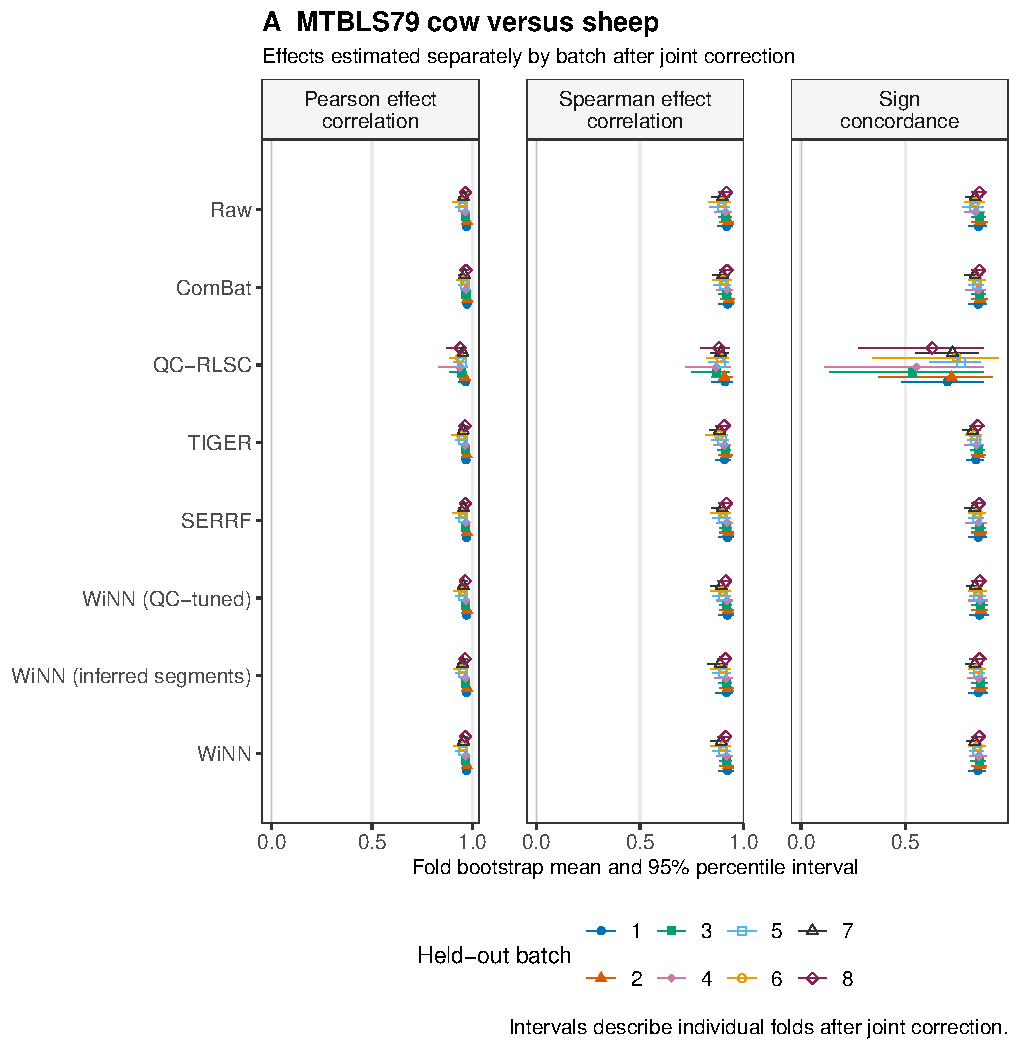
\includegraphics[width=\textwidth]{S7A_lobo_mtbls79_cow_vs_sheep.pdf}
\caption{Cross-batch effect agreement after joint correction for eight outputs. (A) MTBLS79 cow versus sheep. Fold bootstrap means and fold-specific percentile intervals are shown for Pearson effect correlation, Spearman effect correlation and sign concordance. Symbols identify the held-out batch and are displaced vertically only for readability. Every fold uses 2,000 biological-unit resamples conditional on the jointly fitted correction; non-estimable folds remain in the source table.}
\label{fig:supp_lobo}
\end{figure*}

\begin{figure*}[p]
\centering
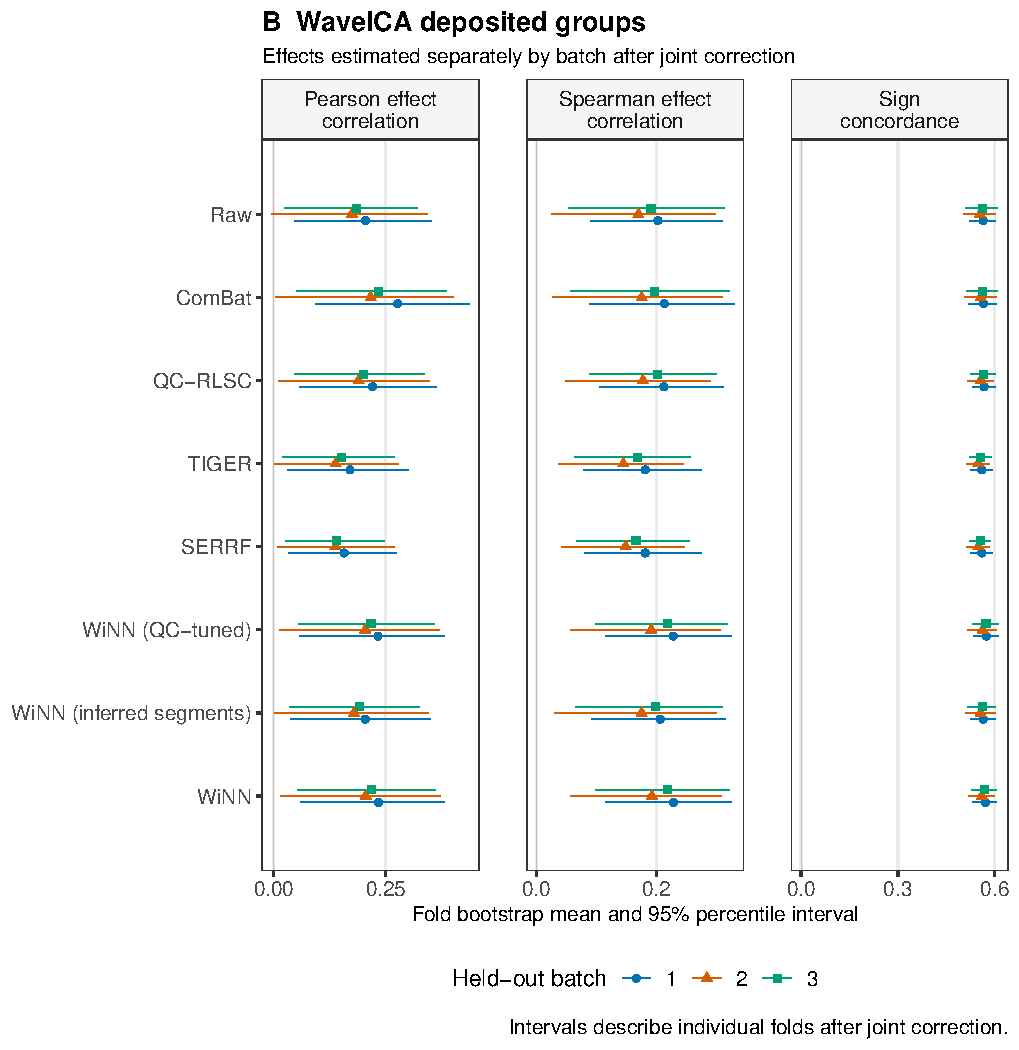
\includegraphics[width=\textwidth]{S7B_lobo_waveica_biological_group.pdf}
\addtocounter{figure}{-1}
\caption{Cross-batch effect agreement after joint correction (continued). (B) WaveICA deposited groups. Points and intervals represent individual batch folds as in panel A.}
\end{figure*}

\begin{figure*}[p]
\centering
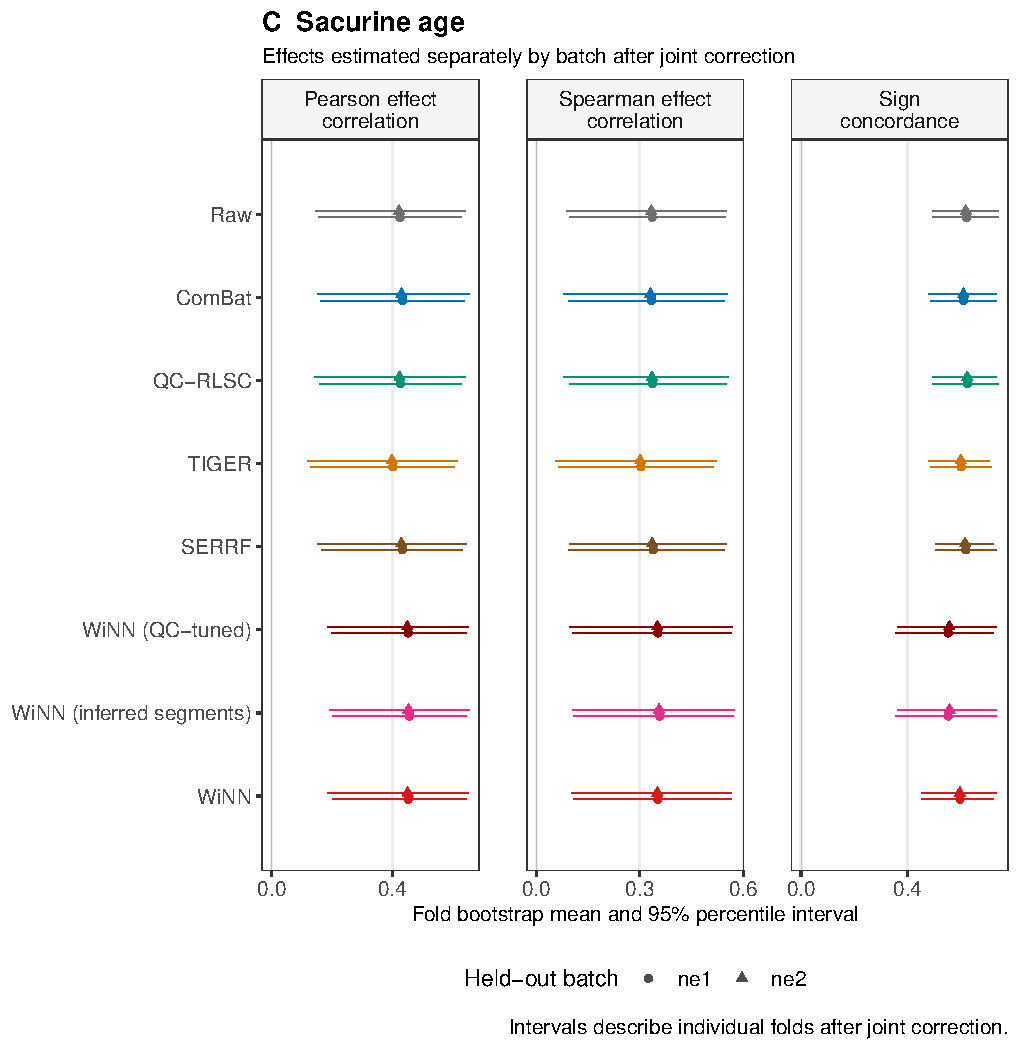
\includegraphics[width=\textwidth]{S7C_lobo_sacurine_age.pdf}
\addtocounter{figure}{-1}
\caption{Cross-batch effect agreement after joint correction (continued). (C) Sacurine age. Only two reciprocal batch comparisons are available. Points and intervals represent individual folds as in panel A.}
\end{figure*}

\begin{figure*}[p]
\centering
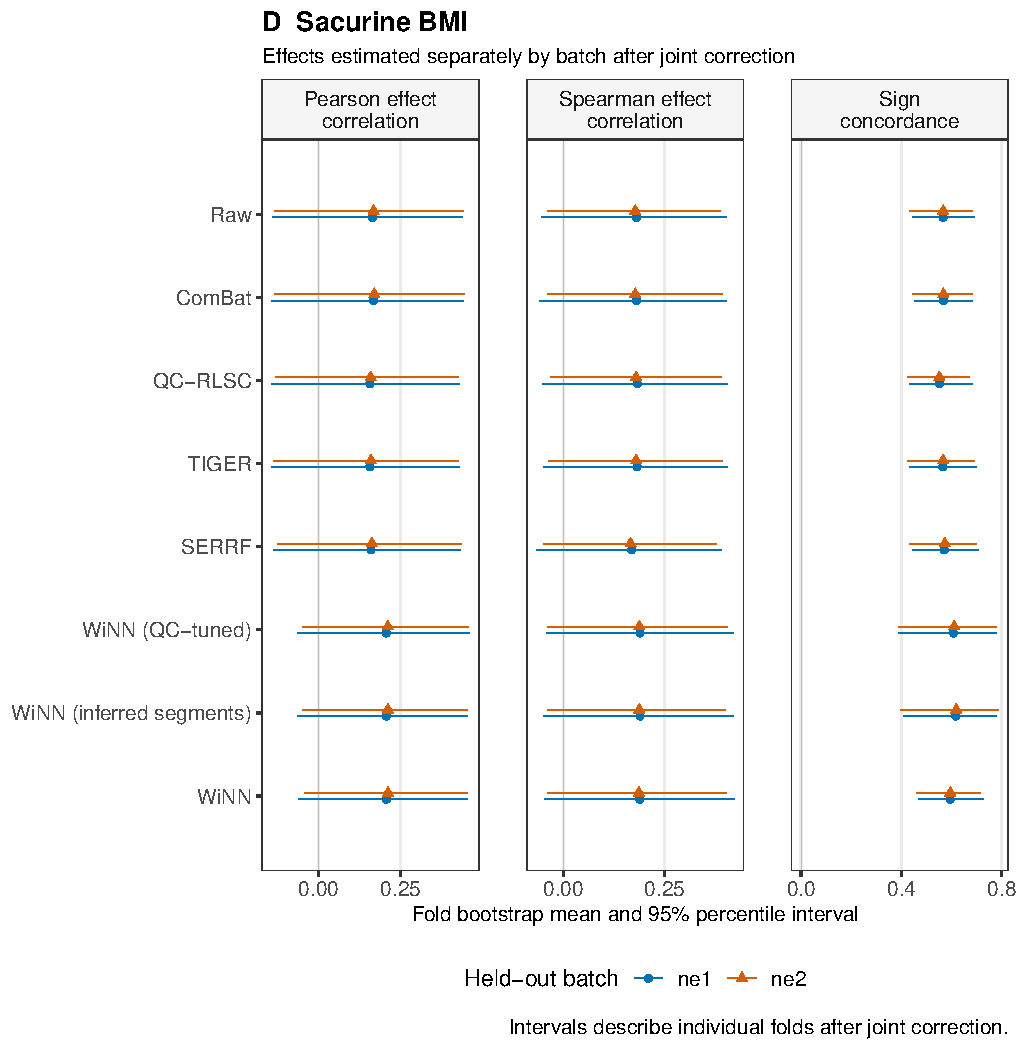
\includegraphics[width=\textwidth]{S7D_lobo_sacurine_bmi.pdf}
\addtocounter{figure}{-1}
\caption{Cross-batch effect agreement after joint correction (continued). (D) Sacurine BMI. Only two reciprocal batch comparisons are available. Points and intervals represent individual folds as in panel A.}
\end{figure*}

\begin{figure*}[p]
\centering
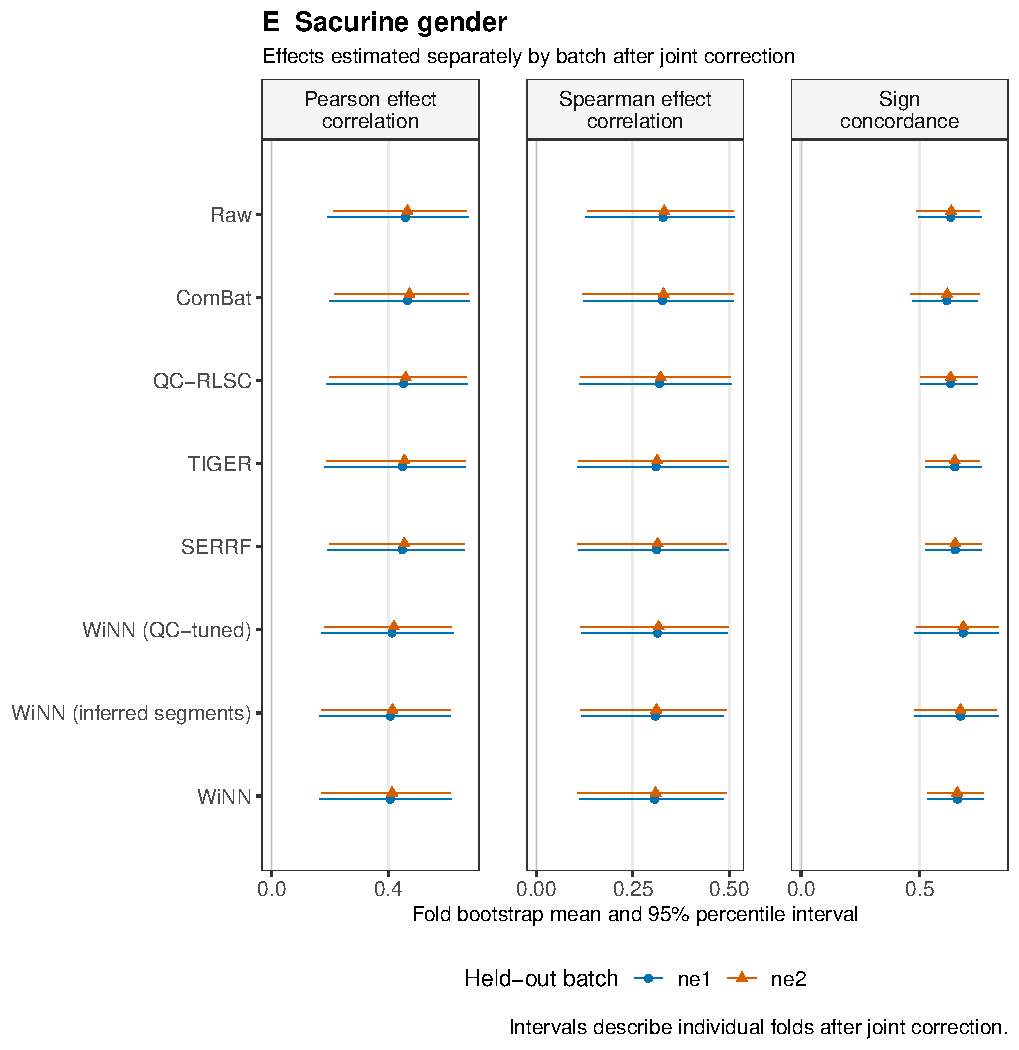
\includegraphics[width=\textwidth]{S7E_lobo_sacurine_gender.pdf}
\addtocounter{figure}{-1}
\caption{Cross-batch effect agreement after joint correction (continued). (E) Sacurine gender. Only two reciprocal batch comparisons are available. Points and intervals represent individual folds as in panel A.}
\end{figure*}

\begin{figure*}[p]
\centering
\supppanel{0.49\textwidth}{S8A_batchcorr_set1_batch_weighted_pc_r2_categorical.pdf}\hfill
\supppanel{0.49\textwidth}{S8B_batchcorr_set1_sample_replicate_pearson_median.pdf}\\[1mm]
\supppanel{0.49\textwidth}{S8C_batchcorr_set1_genuine_replicate_icc_median.pdf}\hfill
\supppanel{0.49\textwidth}{S8D_clinical_fiams_batch_weighted_pc_r2_categorical.pdf}\\[1mm]
\supppanel{0.49\textwidth}{S8E_clinical_fiams_sample_replicate_pearson_median.pdf}\hfill
\supppanel{0.49\textwidth}{S8F_clinical_fiams_genuine_replicate_icc_median.pdf}
\caption{Replicate-profile agreement and technical structure for eight outputs. BatchCorr Set 1 panels show (A) categorical batch \(R^2\), (B) replicate-profile Pearson correlation and (C) within-accession feature-profile ICC(A,1). Clinical FIA-MS panels show (D) categorical plate \(R^2\), (E) replicate-profile Pearson correlation and (F) within-identity feature-profile ICC(A,1). Features are ICC targets and repeated acquisitions are measurement columns within each identity. Points and 95\% intervals use the same 2,000 accession- or identity-cluster bootstrap resamples for every method, conditional on the corrected matrices. The clinical WiNN plate \(R^2\) point is 0.002094, whereas its bootstrap mean is 0.01414 and percentile interval is 0.007357--0.02337. This upward displacement is consistent with resampling bias of in-sample \(R^2\) near zero; the reported intervals are uncorrected percentile intervals.}
\label{fig:supp_replicates}
\end{figure*}

\begingroup
\begin{landscape}
\tiny
\begin{longtable}{lllrrrrrrr}
\caption{Complete biological-association and constrained-permutation results across eight outputs. Null summaries use 5,000 permutations. Association counts are descriptive because ground-truth associated features are unknown in these public datasets.}\label{tab:supp_association}\\
\toprule
Dataset & Endpoint & Method & Tested & BH sig. & Abs. effect & Std. effect & Variance & Null 95th & Empirical $P$ \\
\midrule
\endfirsthead
\multicolumn{10}{l}{\textit{Table \thetable{} continued}}\\
\toprule
Dataset & Endpoint & Method & Tested & BH sig. & Abs. effect & Std. effect & Variance & Null 95th & Empirical $P$ \\
\midrule
\endhead
\midrule
\multicolumn{10}{r}{\textit{Continued on next page}}\\
\endfoot
\bottomrule
\endlastfoot
MTBLS79 & cow vs sheep & Raw & 2488 & 1075 & 0.215 & 0.928 & 0.054 & 0 & <0.001 \\
MTBLS79 & cow vs sheep & ComBat & 2488 & 1095 & 0.216 & 0.957 & 0.050 & 0 & <0.001 \\
MTBLS79 & cow vs sheep & QC-RLSC & 2488 & 284 & 0.222 & 0.366 & 0.370 & 0 & 0.002 \\
MTBLS79 & cow vs sheep & TIGER & 2488 & 1038 & 0.202 & 0.910 & 0.050 & 0 & <0.001 \\
MTBLS79 & cow vs sheep & SERRF & 2488 & 1090 & 0.217 & 0.946 & 0.051 & 0 & <0.001 \\
MTBLS79 & cow vs sheep & WiNN (QC-tuned) & 2488 & 1102 & 0.206 & 0.960 & 0.049 & 0 & <0.001 \\
MTBLS79 & cow vs sheep & WiNN (inferred segments) & 2488 & 1085 & 0.206 & 0.975 & 0.050 & 0 & <0.001 \\
MTBLS79 & cow vs sheep & WiNN & 2488 & 1097 & 0.213 & 0.958 & 0.049 & 0 & <0.001 \\
WaveICA & group 0 vs 1 & Raw & 6461 & 206 & 0.054 & 0.082 & 0.420 & 0 & <0.001 \\
WaveICA & group 0 vs 1 & ComBat & 6461 & 371 & 0.056 & 0.106 & 0.271 & 1 & <0.001 \\
WaveICA & group 0 vs 1 & QC-RLSC & 6461 & 432 & 0.054 & 0.111 & 0.253 & 2 & <0.001 \\
WaveICA & group 0 vs 1 & TIGER & 6461 & 262 & 0.053 & 0.099 & 0.270 & 1 & <0.001 \\
WaveICA & group 0 vs 1 & SERRF & 6461 & 329 & 0.053 & 0.104 & 0.247 & 2 & <0.001 \\
WaveICA & group 0 vs 1 & WiNN (QC-tuned) & 6461 & 485 & 0.053 & 0.123 & 0.199 & 2 & <0.001 \\
WaveICA & group 0 vs 1 & WiNN (inferred segments) & 6461 & 417 & 0.053 & 0.114 & 0.216 & 1 & <0.001 \\
WaveICA & group 0 vs 1 & WiNN & 6461 & 494 & 0.052 & 0.122 & 0.199 & 2 & <0.001 \\
Sacurine & BMI & Raw & 113 & 0 & 0.057 & 0.061 & 0.881 & 0 & 1.000 \\
Sacurine & BMI & ComBat & 113 & 1 & 0.052 & 0.057 & 0.826 & 0 & 0.032 \\
Sacurine & BMI & QC-RLSC & 113 & 0 & 0.054 & 0.070 & 0.763 & 0 & 1.000 \\
Sacurine & BMI & TIGER & 113 & 1 & 0.057 & 0.065 & 0.745 & 0 & 0.033 \\
Sacurine & BMI & SERRF & 113 & 1 & 0.056 & 0.062 & 0.780 & 0 & 0.033 \\
Sacurine & BMI & WiNN (QC-tuned) & 113 & 1 & 0.076 & 0.091 & 0.676 & 0 & 0.036 \\
Sacurine & BMI & WiNN (inferred segments) & 113 & 3 & 0.079 & 0.092 & 0.669 & 0 & 0.012 \\
Sacurine & BMI & WiNN & 113 & 5 & 0.071 & 0.081 & 0.592 & 0 & 0.004 \\
Sacurine & age & Raw & 113 & 16 & 0.098 & 0.098 & 0.881 & 0 & <0.001 \\
Sacurine & age & ComBat & 113 & 18 & 0.096 & 0.104 & 0.826 & 0 & 0.002 \\
Sacurine & age & QC-RLSC & 113 & 23 & 0.098 & 0.119 & 0.763 & 0 & <0.001 \\
Sacurine & age & TIGER & 113 & 15 & 0.085 & 0.096 & 0.745 & 0 & <0.001 \\
Sacurine & age & SERRF & 113 & 17 & 0.096 & 0.094 & 0.780 & 0 & 0.001 \\
Sacurine & age & WiNN (QC-tuned) & 113 & 19 & 0.068 & 0.081 & 0.676 & 0 & 0.004 \\
Sacurine & age & WiNN (inferred segments) & 113 & 18 & 0.068 & 0.080 & 0.669 & 0 & 0.004 \\
Sacurine & age & WiNN & 113 & 23 & 0.091 & 0.111 & 0.592 & 0 & <0.001 \\
Sacurine & gender & Raw & 113 & 14 & 0.230 & 0.226 & 0.881 & 0 & 0.002 \\
Sacurine & gender & ComBat & 113 & 15 & 0.226 & 0.234 & 0.826 & 0 & 0.002 \\
Sacurine & gender & QC-RLSC & 113 & 14 & 0.198 & 0.202 & 0.763 & 0 & 0.001 \\
Sacurine & gender & TIGER & 113 & 16 & 0.225 & 0.256 & 0.745 & 0 & 0.001 \\
Sacurine & gender & SERRF & 113 & 23 & 0.230 & 0.258 & 0.780 & 0 & <0.001 \\
Sacurine & gender & WiNN (QC-tuned) & 113 & 29 & 0.239 & 0.300 & 0.676 & 0 & 0.002 \\
Sacurine & gender & WiNN (inferred segments) & 113 & 27 & 0.241 & 0.287 & 0.669 & 0 & 0.003 \\
Sacurine & gender & WiNN & 113 & 24 & 0.222 & 0.280 & 0.592 & 0 & <0.001 \\
\end{longtable}
\end{landscape}

\endgroup
\begingroup
\scriptsize
\begin{longtable}{llrrr}
\caption{Same-feature effects relative to input abundance. Slope is the through-origin least-squares slope of corrected on input feature effects. Sign concordance and Pearson correlation use matched finite features. Effects use the log1p scale and the dataset-specific osmolality adjustment.}\label{tab:supp_paired_effects}\\
\toprule
Dataset / endpoint & Method & Slope & Sign agreement & Pearson \\
\midrule
\endfirsthead
\toprule
Dataset / endpoint & Method & Slope & Sign agreement & Pearson \\
\midrule
\endhead
\bottomrule
\endlastfoot
MTBLS79 cow--sheep & ComBat & 0.984 & 0.979 & 1.000 \\
MTBLS79 cow--sheep & QC-RLSC & 1.006 & 0.856 & 0.999 \\
MTBLS79 cow--sheep & TIGER & 0.964 & 0.959 & 0.998 \\
MTBLS79 cow--sheep & SERRF & 0.993 & 0.971 & 1.000 \\
MTBLS79 cow--sheep & WiNN (QC-tuned) & 0.981 & 0.971 & 0.999 \\
MTBLS79 cow--sheep & WiNN (inferred segments) & 0.977 & 0.967 & 0.999 \\
MTBLS79 cow--sheep & WiNN & 0.980 & 0.969 & 0.999 \\
WaveICA groups & ComBat & 0.945 & 0.942 & 0.973 \\
WaveICA groups & QC-RLSC & 0.995 & 0.991 & 1.000 \\
WaveICA groups & TIGER & 0.980 & 0.935 & 0.986 \\
WaveICA groups & SERRF & 1.000 & 0.936 & 0.967 \\
WaveICA groups & WiNN (QC-tuned) & 0.964 & 0.914 & 0.993 \\
WaveICA groups & WiNN (inferred segments) & 0.965 & 0.968 & 0.995 \\
WaveICA groups & WiNN & 0.968 & 0.955 & 0.993 \\
Sacurine age & ComBat & 0.988 & 0.991 & 0.999 \\
Sacurine age & QC-RLSC & 1.003 & 0.956 & 0.999 \\
Sacurine age & TIGER & 0.938 & 0.956 & 0.996 \\
Sacurine age & SERRF & 0.987 & 0.982 & 0.998 \\
Sacurine age & WiNN (QC-tuned) & 0.904 & 0.867 & 0.995 \\
Sacurine age & WiNN (inferred segments) & 0.900 & 0.858 & 0.995 \\
Sacurine age & WiNN & 0.937 & 0.973 & 0.994 \\
Sacurine bmi & ComBat & 0.966 & 0.973 & 0.997 \\
Sacurine bmi & QC-RLSC & 0.975 & 0.929 & 0.990 \\
Sacurine bmi & TIGER & 0.984 & 0.982 & 0.997 \\
Sacurine bmi & SERRF & 1.000 & 0.973 & 0.996 \\
Sacurine bmi & WiNN (QC-tuned) & 1.010 & 0.903 & 0.989 \\
Sacurine bmi & WiNN (inferred segments) & 1.012 & 0.885 & 0.983 \\
Sacurine bmi & WiNN & 0.959 & 0.938 & 0.982 \\
Sacurine gender & ComBat & 0.997 & 0.973 & 0.999 \\
Sacurine gender & QC-RLSC & 0.946 & 0.965 & 0.997 \\
Sacurine gender & TIGER & 0.990 & 0.947 & 0.998 \\
Sacurine gender & SERRF & 1.007 & 0.929 & 0.998 \\
Sacurine gender & WiNN (QC-tuned) & 0.923 & 0.885 & 0.974 \\
Sacurine gender & WiNN (inferred segments) & 0.912 & 0.894 & 0.973 \\
Sacurine gender & WiNN & 0.870 & 0.929 & 0.973 \\
\end{longtable}

\endgroup
\begingroup
\begin{landscape}
\footnotesize
\begin{longtable}{p{2.7cm}p{3.4cm}p{4.3cm}p{4.3cm}p{4.8cm}}
\caption{Cross-batch identity discrimination. Estimates and paired biological-identity bootstrap percentile intervals retain eligible-query counts within every resampled identity (2,000 draws). The correlation candidate set and fitted corrections remain fixed. BatchCorr uses 693 eligible queries from 346 identities; clinical FIA-MS uses 536 correction-unit queries from 267 identities. Top-1 accuracy and mean reciprocal rank (MRR) use Pearson similarity of log1p profiles in other batches. The final column is WiNN minus comparator.}\label{tab:supp_identity_retrieval}\\
\toprule
Dataset & Method & Top-1 accuracy [95\% interval] & MRR [95\% interval] & Paired top-1 difference [95\% interval] \\
\midrule
\endfirsthead
\toprule
Dataset & Method & Top-1 accuracy [95\% interval] & MRR [95\% interval] & Paired top-1 difference [95\% interval] \\
\midrule
\endhead
\bottomrule
\endlastfoot
BatchCorr Set 1 & Raw & 0.463 [0.413, 0.513] & 0.528 [0.481, 0.574] & 0.247 [0.204, 0.292] \\
BatchCorr Set 1 & ComBat & 0.716 [0.672, 0.761] & 0.772 [0.734, 0.809] & -0.006 [-0.028, 0.016] \\
BatchCorr Set 1 & QC-RLSC & 0.713 [0.669, 0.757] & 0.768 [0.729, 0.805] & -0.003 [-0.025, 0.018] \\
BatchCorr Set 1 & TIGER & 0.694 [0.648, 0.741] & 0.754 [0.716, 0.795] & 0.016 [-0.013, 0.044] \\
BatchCorr Set 1 & SERRF & 0.693 [0.647, 0.737] & 0.753 [0.714, 0.792] & 0.017 [-0.006, 0.041] \\
BatchCorr Set 1 & WiNN (QC-tuned) & 0.707 [0.662, 0.751] & 0.763 [0.724, 0.802] & 0.003 [-0.006, 0.012] \\
BatchCorr Set 1 & WiNN (inferred segments) & 0.703 [0.658, 0.746] & 0.758 [0.719, 0.795] & 0.007 [-0.009, 0.025] \\
BatchCorr Set 1 & WiNN & 0.710 [0.665, 0.755] & 0.765 [0.726, 0.804] & Reference \\
BatchCorr Set 1 & Mean-only batch & 0.703 [0.656, 0.749] & 0.762 [0.723, 0.800] & 0.007 [-0.014, 0.030] \\
BatchCorr Set 1 & Study-sample ANCOVA & 0.726 [0.682, 0.770] & 0.779 [0.741, 0.816] & -0.016 [-0.037, 0.004] \\
Clinical FIA-MS & Raw & 0.752 [0.706, 0.795] & 0.794 [0.751, 0.832] & 0.110 [0.069, 0.153] \\
Clinical FIA-MS & ComBat & 0.847 [0.807, 0.884] & 0.874 [0.840, 0.906] & 0.015 [-0.007, 0.039] \\
Clinical FIA-MS & QC-RLSC & 0.854 [0.813, 0.891] & 0.878 [0.842, 0.910] & 0.007 [-0.017, 0.032] \\
Clinical FIA-MS & TIGER & 0.881 [0.845, 0.914] & 0.913 [0.885, 0.937] & -0.019 [-0.049, 0.007] \\
Clinical FIA-MS & SERRF & 0.877 [0.843, 0.909] & 0.902 [0.874, 0.928] & -0.015 [-0.043, 0.015] \\
Clinical FIA-MS & WiNN (QC-tuned) & 0.862 [0.824, 0.899] & 0.881 [0.846, 0.913] & 0.000 [-0.006, 0.006] \\
Clinical FIA-MS & WiNN (inferred segments) & 0.858 [0.819, 0.895] & 0.880 [0.843, 0.912] & 0.004 [-0.007, 0.017] \\
Clinical FIA-MS & WiNN & 0.862 [0.824, 0.897] & 0.881 [0.847, 0.913] & Reference \\
Clinical FIA-MS & Mean-only batch & 0.854 [0.816, 0.889] & 0.877 [0.843, 0.908] & 0.007 [-0.019, 0.035] \\
Clinical FIA-MS & Study-sample ANCOVA & 0.851 [0.809, 0.888] & 0.876 [0.840, 0.908] & 0.011 [-0.013, 0.037] \\
\end{longtable}
\end{landscape}

\endgroup

\section{Cumulative technical trajectory and numerical validation}
\label{sec:supp_audit_results}

The cumulative categorical batch trajectory showed that residual batch correction accounted for most of the reduction in discrete technical separation, whereas preparation and drift correction could transiently increase categorical separation (Figure~\ref{fig:supp_trajectory}). Batch was explicitly encoded as a factor at every stage. The clinical trajectory used the 536 study pair means, matching the main-manuscript endpoint.

Dataset-specific automatic-mode parameters are reported in Table~\ref{tab:supp_selected_parameters}. All declared feature and sample panels were complete, and runtime was reported only for fits rerun under the benchmark timing policy (Table~\ref{tab:supp_runtime}). Twenty-two of 684 correction runs required negative extrapolated intensities to be floored at zero, affecting 54,852 values in 8,072 features. Eleven of 76 TIGER runs returned nonfinite values for 141 values in 60 features; these were restored to their raw values and every event was recorded. Dataset--method safeguard counts and the prespecified analyses that were not estimable under the available designs are provided as source data.

All batch $R^2$ computations use categorical coding. A 19-item release validation, combining the WiNN 0.1.6 re-run with the validated comparator outputs, verifies the declared sample and feature panels, separation of training and hidden references, the frozen package identity and finite non-negative corrected matrices; it is provided with the source data.

\begin{figure*}[p]
\centering
\supppanel{0.49\textwidth}{S9A_batch_r2_simulation.pdf}\hfill
\supppanel{0.49\textwidth}{S9B_batch_r2_mtbls79.pdf}\\[1mm]
\supppanel{0.49\textwidth}{S9C_batch_r2_clinical_fiams.pdf}\hfill
\supppanel{0.49\textwidth}{S9D_batch_r2_batchcorr_set1.pdf}\\[1mm]
\supppanel{0.49\textwidth}{S9E_batch_r2_sacurine.pdf}\hfill
\supppanel{0.49\textwidth}{S9F_batch_r2_waveica.pdf}
\caption{Categorical batch weighted-PC \(R^2\) through the WiNN cumulative workflow in (A) simulation, (B) MTBLS79, (C) clinical FIA-MS, (D) BatchCorr Set 1, (E) Sacurine and (F) WaveICA. Values are computed from raw input and immutable matrices after MAD preparation, selective drift correction, residual batch correction and conservative PQN. Panel A uses the prespecified representative simulation seed, not the ten-seed main-text average.}
\label{fig:supp_trajectory}
\end{figure*}

\begin{figure*}[p]
\centering
\supppanel{\textwidth}{S10A_sacurine_age_weighted_pc_r2.pdf}\\[1mm]
\supppanel{\textwidth}{S10B_sacurine_bmi_weighted_pc_r2.pdf}\\[1mm]
\supppanel{\textwidth}{S10C_sacurine_gender_weighted_pc_r2.pdf}
\caption{Sacurine technical-biological trade-offs for eight outputs: (A) age, (B) BMI and (C) gender. The horizontal axis is categorical batch weighted-PC \(R^2\) from the pre-osmolality correction output; the vertical axis is covariate weighted-PC \(R^2\) after each corrected study profile is divided by sample osmolality and transformed as \(\log(1+x)\). Points are full-sample estimates and bars are bootstrap standard errors from 2,000 batch-stratified study-sample resamples. Axes are scaled separately by covariate.}
\label{fig:supp_sacurine}
\end{figure*}



\section{Gate calibration, biological stress tests and additional baselines}
\label{sec:supp_targeted_revision}

\subsection{Technical-gate calibration}

We evaluated technical-gate calibration using WiNN 0.1.6. Scripts and seed-level results are supplied in \path{scripts/targeted_validation/} and \path{generated/review_validation/}. A deterministic sequence with study log1p values one and every tenth QC value zero has zero MAD, unchanged preparation, lag-10 autocorrelation 0.9 and a lag-10 contribution of 91.8 to the Ljung--Box statistic. Scheduled sample-type differences therefore trigger the gate even in the absence of instrumental drift.

An independent null experiment generated 100 Gaussian log1p feature profiles per segment, with mean three and standard deviation 0.15, at segment lengths 20, 50, 100 and 200, using 1,000 seeds at each length. The adaptive lag is four at length 20 and ten at the other lengths. Each seed applies the Ljung--Box gate and BH adjustment at nominal 0.05 across all 100 null features. Before MAD preparation, the probabilities of any false rejection were 0.131, 0.350, 0.197 and 0.122, respectively; exact binomial 95\% Monte Carlo intervals were [0.111, 0.154], [0.320, 0.380], [0.173, 0.223] and [0.102, 0.144]. Under this global null, the probability of any rejection equals the empirical FDR. The corresponding mean numbers of rejected features were 0.161, 0.498, 0.241 and 0.142 out of 100. After MAD preparation, empirical FDR was 0.135, 0.349, 0.198 and 0.123. The vectorized implementation agreed with R's \texttt{Box.test} to $10^{-12}$ for every feature of the first ten seeds at each length. The approximate Ljung--Box reference was therefore anticonservative at these segment lengths; MAD preparation had little effect on the result.

Additional 100-seed experiments varied feature correlation (zero or 0.6), regularly interleaved QC mean shifts and drift in 20 of 100 features. A batch-gate experiment used four balanced batches of 25 injections, with or without repeated identities and with or without batch offsets in 20 features, before and after selective detrending. Seed-level sensitivity, false-discovery proportions and null-tail summaries are supplied for each design.

\subsection{Biological stress tests for ungated preparation and PQN}

Artifact-free simulations used 200 features and 200 samples, random subgroup allocation, feature baseline log intensities spanning two to five, independent log noise of standard deviation 0.12 and a shared random sample component of standard deviation 0.08. Each of 100 seeds compared raw input, MAD alone, conservative PQN alone and MAD followed by PQN. A balanced sparse response affected 40 features in half of samples, with 20 effects of $+0.7$ and 20 of $-0.7$ on the generating log scale. A rare subgroup affected 5\% of samples and 40 features, all with $+1.4$ effects. A broad coordinated response affected 20\% of samples and 160 features, all with $+0.7$ effects. Recovery was evaluated as the feature-median signed corrected-to-clean effect ratio on the same log1p scale, then averaged over seeds.

Table~\ref{tab:supp_stage_response_patterns} separates the preparation and dilution stages. MAD followed by PQN retained a mean recovery ratio of 1.000 in the balanced sparse design, 0.310 in the rare subgroup design and 0.534 in the broad coordinated design. For rare subgroups, MAD alone gave 0.319 and PQN alone 0.991; for broad coordinated responses they gave 0.778 and 0.711. MAD shrinkage thus attenuated rare responses, while both preparation and PQN attenuated broad coordinated responses. These artifact-free experiments identify the biological patterns affected by each stage independently of technical correction.

\subsection{Study-sample regression baselines}

We ran the Wehrens study-sample ANCOVA implementation \citep{Wehrens2016BatchCorr} from \texttt{BatchCorrMetabolomics} 0.1.14 at commit \texttt{e0c7668}. Feature-wise \texttt{doBC} fits used \texttt{method="lm"}, log1p intensity, supplied batch factors and acquisition-order slopes with batch interactions ($X\sim S*B$). The primary baseline uses all injections and the same intensity, acquisition-order and batch information as WiNN. Mean-only batch adjustment omits acquisition order. A study-only ANCOVA sensitivity analysis additionally uses reference/study identities to select the fitting observations. Outputs were inverse-transformed with expm1, and negative extrapolations were floored at zero.

All-injection ANCOVA reduced held-out mean CV from 28.757\% to 17.054\% in MTBLS79, 66.570\% to 29.023\% in BatchCorr, 16.594\% to 15.582\% in the clinical data, 32.599\% to 18.072\% in Sacurine and 49.662\% to 40.652\% in WaveICA (Table~\ref{tab:supp_baselines}B). WaveICA all-injection ANCOVA required flooring 4,601 cells, and mean-only adjustment required flooring 6,722 cells. Public inputs match the benchmark input hashes. The clinical input was reconstructed from pair-level data; its raw plate $R^2$ agrees with the original estimate to approximately $10^{-12}$ (0.1505094553797 versus 0.1505094553801). Clinical baseline results use this reconstruction rather than a byte-identical copy of the original matrix.

On the ten canonical simulation inputs, mean-only batch adjustment gave mean clean-truth RMSE 0.1164, feature-profile ICC 0.8487 and sample-profile correlation 0.8454; study-sample ANCOVA gave 0.0981, 0.8870 and 0.8842. WiNN gave 0.0722, 0.9231 and 0.9247 and improved all three endpoints in every paired seed (Table~\ref{tab:supp_baselines}A). The simulation input and clean-truth hashes match the original ten-seed benchmark.

Empirical comparisons use the same independent biological units and covariate models as the primary analyses (Table~\ref{tab:supp_baselines}C). Mean-only batch adjustment and ANCOVA retained raw feature-effect magnitudes more closely for several contrasts: their WaveICA slopes were both 0.994 versus 0.968 for WiNN, and Sacurine gender slopes were 1.006 and 0.970 versus 0.871. Raw effects provide an observed reference, not biological ground truth. Paired top-1 retrieval differences between WiNN and each baseline included zero in both repeated-identity datasets (Table~\ref{tab:supp_identity_retrieval}). The simulation advantage therefore did not imply uniform superiority on empirical biological endpoints.

\subsection{Paired empirical feature effects and acquisition design}

Table~\ref{tab:supp_paired_effects} reports matched-feature slopes and sign agreement for the eight empirical outputs relative to raw input. WiNN slopes were 0.980 for MTBLS79, 0.968 for WaveICA and 0.936, 0.969 and 0.871 for Sacurine age, BMI and gender. Corresponding sign-agreement fractions were 0.969, 0.951, 0.973, 0.947 and 0.929. These paired summaries quantify changes relative to the observed uncorrected effects.

Table~\ref{tab:supp_acquisition_balance} reports group-by-batch counts; reference placement within each batch is provided in \path{generated/review_validation/prepared_design_reference_placement.csv}. Additional summaries provide repeated-identity placement and covariate balance with run order in \path{generated/review_validation/prepared_design_*.csv}. The WaveICA batch counts are 24/168, 24/168 and 23/161 for deposited groups 0/1, showing similar group proportions in each batch despite the overall imbalance. MTBLS79 cow/sheep counts vary across batches, and Sacurine female/male counts are 46/44 and 37/57 in its two batches. The clinical analysis has 80, 78, 55, 55, 80, 79, 55 and 54 study pair units across eight plates, with cross-plate identity matches available. The clinical dataset provides repeated identities without phenotype labels.

\subsection{Practical operating guidance}

Before fitting WiNN, examine group allocation and continuous covariates across analytical batches and acquisition order, and distinguish study injections from scheduled reference types. The all-injection serial-dependence screen can select a profile because of a periodic reference--study difference, even when study-sample order is randomized. In that setting, compare an explicitly reference-trained or batch-only correction using independent biological assessments. Treat the Ljung--Box threshold as a heuristic selection parameter, not a calibrated guarantee of technical-effect FDR.

The primary preparation and PQN configuration is inappropriate when rare-subgroup abundance changes or widespread coordinated shifts are the biological target. The stage experiment attributes most rare-subgroup attenuation to MAD shrinkage; both MAD and PQN attenuate the broad coordinated response. The public \texttt{winn()} entry point always applies MAD preparation. In prespecified mode, \texttt{median\_adjustment="none"} disables PQN, but leaves MAD preparation active. Rare-subgroup attenuation therefore remains active. Select an alternative preparation/correction workflow and validate it against known biological contrasts when these response patterns are expected.

Acquisition-quartile group counts are supplied in \path{generated/review_validation/design_group_acquisition_quartiles.csv}. Sacurine covariate medians and interquartile ranges by batch and acquisition quartile are in \path{generated/review_validation/design_covariate_acquisition_quartiles.csv}. Within-batch age--order Spearman correlations were $-0.110$ and $-0.065$, and BMI--order correlations were $-0.117$ and $0.045$. The clinical metadata contain repeated identities and reference roles but no phenotype variables; phenotype--acquisition balance cannot be assessed for that cohort.

\begingroup
\begin{landscape}
\footnotesize
\begin{longtable}{p{3.0cm}p{3.6cm}rrrrr}
\caption{Same-information baselines. Mean-only batch centering and the Wehrens study-sample ANCOVA use all injections with the same intensity, acquisition-order and batch information as WiNN; the study-only ANCOVA additionally uses reference identities to choose fitting observations. (A) Ten-seed ground-truth endpoints; WiNN advantages are comparator minus WiNN for RMSE and WiNN minus comparator otherwise, with 95\% $t_9$ intervals, and WiNN improved every endpoint in every seed. (B) Held-out QC CV, variance explained by batch (weighted-PC $R^2$) among study injections and negative extrapolations floored at zero. (C) Through-origin slope, sign agreement and Pearson correlation of corrected against raw feature effects, median leave-one-batch-out effect correlation and BH-significant feature counts. Raw effects are an observed reference, not biological truth.}\label{tab:supp_baselines}\\
\toprule
\endfirsthead
\multicolumn{7}{l}{\textit{Table \thetable{} continued}}\\
\toprule
\endhead
\midrule
\multicolumn{7}{r}{\textit{Continued on next page}}\\
\endfoot
\bottomrule
\endlastfoot
\multicolumn{7}{l}{\textbf{A. Simulation truth (ten seeds; mean $\pm$ SE)}} \\
 & \textit{Method} & \textit{Held-out QC CV (\%)} & \textit{RMSE} & \textit{Feature ICC} & \textit{Sample $r$} &  \\
\midrule
Simulation & Raw & $44.550 \pm 0.285$ & $0.2927 \pm 0.0015$ & $0.5879 \pm 0.0020$ & $0.5189 \pm 0.0021$ &  \\
Simulation & Mean-only batch & $15.623 \pm 0.193$ & $0.1164 \pm 0.0004$ & $0.8487 \pm 0.0008$ & $0.8454 \pm 0.0008$ &  \\
Simulation & Study-sample ANCOVA & $12.695 \pm 0.134$ & $0.0981 \pm 0.0004$ & $0.8870 \pm 0.0006$ & $0.8842 \pm 0.0008$ &  \\
Simulation & WiNN & $8.415 \pm 0.057$ & $0.0722 \pm 0.0004$ & $0.9231 \pm 0.0005$ & $0.9247 \pm 0.0010$ &  \\
WiNN advantage & over Mean-only batch & --- & 0.044 [0.043, 0.045] & 0.074 [0.073, 0.076] & 0.079 [0.078, 0.081] &  \\
WiNN advantage & over Study-sample ANCOVA & --- & 0.026 [0.025, 0.026] & 0.036 [0.035, 0.037] & 0.041 [0.039, 0.042] &  \\
\midrule
\multicolumn{7}{l}{\textbf{B. Empirical reference precision and batch association}} \\
\textit{Dataset} & \textit{Fit} & \textit{Held-out QC CV (\%)} & \textit{Batch $R^2$} & \textit{Floored cells} &  &  \\
\midrule
MTBLS79 & Raw & 28.757 & 0.36099 & 0 &  &  \\
MTBLS79 & Mean-only, all & 16.619 & 0.01035 & 0 &  &  \\
MTBLS79 & ANCOVA, all & 17.054 & 0.00968 & 0 &  &  \\
MTBLS79 & ANCOVA, study only & 21.078 & 0.00000 & 0 &  &  \\
Clinical FIA-MS & Raw & 16.594 & 0.15051 & 0 &  &  \\
Clinical FIA-MS & Mean-only, all & 14.549 & 0.00168 & 0 &  &  \\
Clinical FIA-MS & ANCOVA, all & 15.582 & 0.00108 & 0 &  &  \\
Clinical FIA-MS & ANCOVA, study only & 16.693 & 0.00000 & 0 &  &  \\
BatchCorr Set 1 & Raw & 66.570 & 0.56111 & 0 &  &  \\
BatchCorr Set 1 & Mean-only, all & 30.611 & 0.00018 & 0 &  &  \\
BatchCorr Set 1 & ANCOVA, all & 29.023 & 0.00021 & 0 &  &  \\
BatchCorr Set 1 & ANCOVA, study only & 30.226 & 0.00000 & 0 &  &  \\
Sacurine & Raw & 32.599 & 0.13166 & 0 &  &  \\
Sacurine & Mean-only, all & 24.934 & 0.00012 & 0 &  &  \\
Sacurine & ANCOVA, all & 18.072 & 0.00013 & 0 &  &  \\
Sacurine & ANCOVA, study only & 19.697 & 0.00000 & 0 &  &  \\
WaveICA & Raw & 49.662 & 0.69437 & 0 &  &  \\
WaveICA & Mean-only, all & 42.823 & 0.00027 & 6722 &  &  \\
WaveICA & ANCOVA, all & 40.652 & 0.00232 & 4601 &  &  \\
WaveICA & ANCOVA, study only & 42.240 & 0.00000 & 4646 &  &  \\
\midrule
\multicolumn{7}{l}{\textbf{C. Matched-feature effects relative to raw input}} \\
\textit{Dataset / endpoint} & \textit{Method} & \textit{Slope} & \textit{Sign agreement} & \textit{Pearson} & \textit{LOBO Pearson} & \textit{BH count} \\
\midrule
MTBLS79 cow--sheep & Raw & 1.000 & 1.000 & 1.000 & 0.977 & 1075 \\
MTBLS79 cow--sheep & Mean-only batch & 0.992 & 0.972 & 1.000 & 0.977 & 1093 \\
MTBLS79 cow--sheep & Study-sample ANCOVA & 0.981 & 0.971 & 1.000 & 0.977 & 1111 \\
MTBLS79 cow--sheep & WiNN & 0.980 & 0.969 & 0.999 & 0.977 & 1097 \\
WaveICA groups & Raw & 1.000 & 1.000 & 1.000 & 0.305 & 206 \\
WaveICA groups & Mean-only batch & 0.994 & 1.000 & 1.000 & 0.306 & 368 \\
WaveICA groups & Study-sample ANCOVA & 0.994 & 0.994 & 1.000 & 0.304 & 445 \\
WaveICA groups & WiNN & 0.968 & 0.951 & 0.993 & 0.311 & 494 \\
Sacurine age & Raw & 1.000 & 1.000 & 1.000 & 0.556 & 16 \\
Sacurine bmi & Raw & 1.000 & 1.000 & 1.000 & 0.298 & 0 \\
Sacurine gender & Raw & 1.000 & 1.000 & 1.000 & 0.637 & 14 \\
Sacurine age & Mean-only batch & 0.999 & 0.991 & 1.000 & 0.559 & 18 \\
Sacurine bmi & Mean-only batch & 0.988 & 0.991 & 0.999 & 0.295 & 1 \\
Sacurine gender & Mean-only batch & 1.006 & 0.973 & 1.000 & 0.641 & 15 \\
Sacurine age & Study-sample ANCOVA & 1.007 & 0.956 & 0.999 & 0.566 & 23 \\
Sacurine bmi & Study-sample ANCOVA & 0.984 & 0.982 & 0.999 & 0.289 & 1 \\
Sacurine gender & Study-sample ANCOVA & 0.970 & 0.947 & 0.992 & 0.623 & 13 \\
Sacurine age & WiNN & 0.936 & 0.973 & 0.995 & 0.588 & 23 \\
Sacurine bmi & WiNN & 0.969 & 0.947 & 0.985 & 0.379 & 5 \\
Sacurine gender & WiNN & 0.871 & 0.929 & 0.975 & 0.581 & 24 \\
\end{longtable}
\end{landscape}

\endgroup
\begingroup
\footnotesize
\begin{longtable}{lrrr}
\caption{Stage-specific biological effect recovery in artifact-free simulations. Each cell is the mean over 100 seeds of the median signed corrected-to-ground-truth effect ratio across responsive features. A ratio of one denotes unchanged effects. These tests isolate preparation and thresholded PQN from drift and batch adjustment.}\label{tab:supp_stage_response_patterns}\\
\toprule
Response design & MAD alone & PQN alone & MAD + PQN \\
\midrule
\endfirsthead
\multicolumn{4}{l}{Table~\thetable\ (continued)} \\
\toprule
Response design & MAD alone & PQN alone & MAD + PQN \\
\midrule
\endhead
\bottomrule
\endlastfoot
Balanced sparse & 1.0000 & 1.0002 & 1.0002 \\
Rare subgroup & 0.3189 & 0.9906 & 0.3099 \\
Broad coordinated & 0.7779 & 0.7106 & 0.5343 \\
\end{longtable}

\endgroup
\begingroup
\footnotesize
\begin{longtable}{llp{60mm}r}
\caption{Biological group counts by analytical batch and linear association with acquisition order. The final column is the ordinary $R^2$ from regressing within-batch run order on the group indicator. C/S denote cow/sheep; Sacurine uses deposited F/M gender labels; WaveICA retains biological groups 0/1. Quartile-level group counts and continuous-covariate medians and interquartile ranges are supplied as aggregate source CSVs.}\label{tab:supp_acquisition_balance}\\
\toprule
Dataset & Batch & Study-group counts & Order $R^2$ \\
\midrule
\endfirsthead
\multicolumn{4}{l}{Table~\thetable\ (continued)} \\
\toprule
Dataset & Batch & Study-group counts & Order $R^2$ \\
\midrule
\endhead
\bottomrule
\endlastfoot
MTBLS79 & 1 & C: 8; S: 8 & 0.0060 \\
MTBLS79 & 2 & C: 10; S: 10 & 0.0034 \\
MTBLS79 & 3 & C: 10; S: 10 & 0.0034 \\
MTBLS79 & 4 & C: 7; S: 9 & 0.0002 \\
MTBLS79 & 5 & C: 7; S: 5 & 0.0136 \\
MTBLS79 & 6 & C: 8; S: 7 & 0.0204 \\
MTBLS79 & 7 & C: 8; S: 9 & 0.0407 \\
MTBLS79 & 8 & C: 8; S: 10 & 0.0134 \\
Sacurine & ne1 & Female: 46; Male: 44 & 0.0892 \\
Sacurine & ne2 & Female: 37; Male: 57 & 0.0162 \\
WaveICA & 1 & group\_0: 24; group\_1: 168 & 0.0000 \\
WaveICA & 2 & group\_0: 24; group\_1: 168 & 0.0000 \\
WaveICA & 3 & group\_0: 23; group\_1: 161 & 0.0000 \\
\end{longtable}

\endgroup

\section{Application to experimental design}
\label{sec:supp_scope}

The benchmarks support selective detrending and residual batch adjustment for randomized acquisition designs. Recorded batch labels are preferred to automatic segmentation. All benchmark datasets contain reference injections; their identities are withheld from WiNN. Replicate-profile agreement, cross-batch identity retrieval and matched-feature effects capture distinct aspects of biological structure. Their use alongside technical endpoints is especially important when biological groups are unevenly distributed across acquisition order or when rare and coordinated responses interact with MAD preparation or PQN.

\bibliographystyle{oup-abbrvnat}
\bibliography{references}
\end{document}
